\documentclass[a4paper,11pt]{article}
\usepackage{eurosym}
\usepackage{bbm}
\usepackage[onehalfspacing]{setspace}
\usepackage{authblk}
\usepackage{pgf}
\usepackage{xcolor}
\usepackage{mathtools}
\usepackage[utf8]{inputenc}
\usepackage{color}
\usepackage{calrsfs}
\usepackage{amsfonts}
\usepackage{amssymb}
\usepackage{amsmath}
\usepackage{amsthm}
\usepackage{cellspace}
\usepackage{caption}
\usepackage{booktabs}
\usepackage{multirow}
\usepackage{listings}
\usepackage[english]{babel}
\usepackage[style = apa]{biblatex}
\DeclareLanguageMapping{english}{english-apa}
\newcommand\poscite[1]{\citeauthor{#1}'s (\citeyear{#1})}
\usepackage[top=2cm,bottom=2.2cm,left=3cm,right=3cm]{geometry}
\usepackage[breaklinks=true,colorlinks=true,linkcolor=blue,citecolor=blue,filecolor=blue,urlcolor=blue]{hyperref}
\allowdisplaybreaks
\mathtoolsset{showonlyrefs}

\definecolor{refcol}{RGB}{0,90,160}
\definecolor{newcol}{RGB}{150,40,40}
\newcommand{\RR}[1]{\textcolor{refcol}{#1}}
\newcommand{\NN}[1]{\textcolor{newcol}{#1}}
\newcommand{\refnote}[1]{\footnote{\textcolor{refcol}{\textsf{\footnotesize #1}}}}


\makeatletter
\renewenvironment{proof}[1][\proofname]{%
  \par\pushQED{\qed}\normalfont%
  \topsep6\p@\@plus6\p@\relax
  \trivlist\item[\hskip\labelsep\bfseries#1\@addpunct{.}]%
  \ignorespaces
}{%
  \popQED\endtrivlist\@endpefalse
}
\makeatother

\newcommand{\R}{\mathbb R}
\newcommand{\E}{\mathbb E}
\renewcommand{\P}{\mathbb P}
\newcommand{\Var}{\operatorname{Var}}
\newcommand{\Cov}{\operatorname{Cov}}
\newcommand{\dd}{\mathrm d}
\newcommand{\RT}{\mathrm{RT}}
\newcommand{\bigO}{\mathcal{O}}
\newcommand{\1}{\mathbbm{1}}
\newcommand{\indep}{\perp\!\!\!\perp}
\DeclareMathOperator{\sgn}{sgn}


\newtheorem{definition}{Definition}
\newtheorem{axiom}{Axiom}
\newtheorem{theorem}{Theorem}
\newtheorem{proposition}{Proposition}
\newtheorem{remark}{Remark}



%% local new commands
\newcommand{\Lmot}{L_{\mathrm{motion}}}
\newcommand{\Lrs}{L_{\mathrm{RS}}}
\newcommand{\Lmo}{L_{\mathrm{motor}}}
\newcommand{\toff}{t_{\mathrm{offset}}}
\newcommand{\trs}{t_{\mathrm{RS}}}
\newcommand{\sresp}{s_{\mathrm{resp}}}




\addbibresource{~/thib/projects/tools/bib_thib_zotero.bib}

\graphicspath{{figures/}}

\title{The extended evidence-accumulation model for delayed reports}
\date{}

\begin{document}
\maketitle


\tableofcontents

%======================================================================
\section{The model}
\label{sec:model}

Time $t$ runs from motion-stimulus onset. Motion of coherence $c$ and direction
$s\in\{-1,+1\}$ is presented for a duration $D$. Encoding time for the motion evidence is
fixed across conditions and equal to $\Lmot$, so encoded motion evidence is available to
the decision process on $[\Lmot,\ \Lmot+D]$.

\subsection{Accumulation}

The decision variable $x$ and the motor-preparatory state $y$ obey
\begin{equation}
\dd x(t)=s\,k\,c\,\dd t+\sigma_x\,\dd W_x(t),
\qquad
\dd y(t)=\lambda\,[x(t)-y(t)]\,\dd t ,
\label{eq:acc}
\end{equation}
where $W_x$ is a standard Wiener process and $\sigma_x$ is taken as a fixed scaling
parameter. Only $kc/\sigma_x$ has meaning: the model is invariant under a common
rescaling of $x$, $y$, $\theta$, $g$, $r$ and the maintenance noise, so one amplitude has
to be declared, and $\sigma_x$ is it.

\subsection{Commitment}

Maintenance begins at
\begin{equation}
\tau:=\inf\{t\in[\Lmot,\toff]:|y(t)|\ge\theta\}\wedge\toff,
\qquad \toff:=D+\Lmot,
\end{equation}
with $\sresp:=\sgn y(\tau)$ and maintenance target
\begin{equation}
m:=\begin{cases}\sresp\,\theta,&\text{if the threshold was reached},\\
y(\toff),&\text{otherwise,}\end{cases}
\label{eq:m}
\end{equation}
where $\theta$ is a threshold smaller than $g$. Note that $y(\tau)=m$ in both branches:
if the threshold is reached, $y$ hits $\theta$ continuously; if it is not, $\tau=\toff$
and $m=y(\toff)$ by definition. The maintained state therefore has no approach transient,
and $m=\sresp|m|$ with $|m|=\min(|y(\toff)|,\theta)$ pathwise.

\subsection{Maintenance}

Let $\trs:=D+3+\Lrs$ be the time at which the response signal is encoded. On
$[\tau,\trs)$ the motor-preparatory state has two parts.

The first is a noisy maintenance of a baseline at the target $m$,
\begin{equation}\label{eq:maint}
\dd y(t)=\lambda\,[m+\varepsilon(t)-y(t)]\,\dd t,
\end{equation}
where
\begin{equation}
\dd\varepsilon(t)=-\kappa\varepsilon(t)\,\dd t+\sigma_\varepsilon\,\dd W_\varepsilon(t),
\quad \varepsilon(\tau)=0,
\end{equation}
is an Ornstein--Uhlenbeck process relaxing to zero at rate $\kappa$, with $W_\varepsilon$
independent of $W_x$, and stationary standard deviation
$\mathrm{SD}_\varepsilon=\sigma_\varepsilon/\sqrt{2\kappa}$. The initial condition and
that standard deviation are not in conflict: $\varepsilon$ starts at zero and its variance
grows as $\mathrm{SD}_\varepsilon^{2}(1-e^{-2\kappa\rho})$, so
$\mathrm{SD}_\varepsilon$ describes the process only once the transient has passed,
which takes a few multiples of $1/2\kappa$. Were $\kappa=0$, that is,
were the noise a Wiener process rather than an Ornstein--Uhlenbeck one, its standard
deviation would grow without bound over the delay.

The second is temporal preparation, added optionally, and modelled as a linear ramp from
zero at $\toff$ to $\beta$ at $\trs$, that is over
$\Delta:=\trs-\toff=3+\Lrs-\Lmot$, at rate $\alpha:=\beta/\Delta$. The signal reaching
the gate is
\begin{equation}
\tilde y(t)=y(t)+\sresp\,\beta\,\min\!\left(1,\frac{(t-\toff)^{+}}{\Delta}\right),
\end{equation}
frozen at $\sresp\beta$ once $t>\trs$, and the neural drive to the selected agonist is
\begin{equation}
z(t)=\max\bigl[\sresp\,\tilde y(t)-g,\,0\bigr].
\label{eq:z}
\end{equation}

\medskip
\noindent\textbf{Model 1 and Model 2.} Model 1 is the case $\beta=0$, with no temporal
preparation; Model 2 is $\beta>0$.

\subsection{Response stage}

At $\trs$ the maintenance noise is discontinued and
\begin{equation}
\dd q(t)=\mu_{\mathrm{RS}}\dd t+\sigma_q\dd W_q(t),\ q(\trs)=0,
\qquad
\dd y(t)=\lambda\,[\,y(\trs)+\sresp\,q(t)-y(t)\,]\,\dd t,
\label{eq:resp}
\end{equation}
where $W_q$ is a Wiener process independent of both $W_x$ and $W_\varepsilon$. The
response is triggered when $z$ reaches $r$, and occurs $\Lmo$ later. An excursion of $z$
above zero that returns to zero without reaching $r$ is a partial activation.

%=====================================================================
\section{Theoretical predictions}
\label{sec:pred}

\subsection{Behaviour}

Behaviour here means what is available without electromyography: accuracy and response
time, that is the first six rows of Table~S1. Responses made before the signal are
excluded from the analyses, and the model treats them as a nuisance rather than a
dependent variable.

\paragraph{Accuracy rises with coherence and with duration (R1, R2).}\footnote{Labels R1
to R27 index the results of Tables~S1 and~S2, reproduced with an added column in
Appendix~\ref{app:obs}.} The choice is fixed at commitment, as the sign of $y(\tau)$, and
nothing after commitment can change it. Accuracy therefore reflects the first
accumulation alone: it rises with coherence because the drift $kc$ is larger relative to
$\sigma_x$, and with duration because the accumulation runs longer before it is stopped.
It is the one measure in the experiment that carries no information about anything
downstream of commitment.

\paragraph{The duration benefit is confined to intermediate coherence (R3).} At zero
coherence there is no signal to accumulate, so more time cannot help; at fifty per cent
the threshold $\theta$ is reached almost at once, so more time is not needed. The benefit
of duration is therefore squeezed into the intermediate level, which is what the
interaction reports. This is a floor-and-ceiling effect and not a mechanism: it requires
only that $\theta$ be reachable within $0.3$~s at high coherence and not at all at zero.

\paragraph{Response time falls with coherence and with duration (R4, R5).} At the response
signal the second accumulation starts at a distance $g-|m|-\beta$ below the gate, and its
drift is the same in every condition. Coherence and duration can therefore act on response
time only through that starting distance. Raising either raises the maintained level
$|m|$ --- higher coherence because the drift is larger, longer duration because
accumulation is stopped later --- which shortens the distance left to travel. Nothing
downstream of the starting point depends on the stimulus.

\paragraph{The coherence effect on response time is larger after a short stimulus (R6).}
The maintained level is capped at $\theta$: a trial that reaches the threshold is held
there whatever its coherence. After a long stimulus most trials reach it at every
coherence, so their starting points are compressed towards a common value and the
coherence effect shrinks; after a short stimulus fewer do, and the starting points spread.
The interaction therefore follows from the cap alone, with no further assumption. It is
worth marking that this same argument, applied to the offset-locked rate, gives the
opposite sign to what is observed there --- see R19 below and
Section~\ref{sec:notfollow}.

\subsection{During the delay}

The four analysis windows are locked to the four trial events and do not coincide with
the intervals they are named after, so this note calls them the \emph{onset-locked},
\emph{offset-locked}, \emph{signal-locked} and \emph{response-locked} windows; their
bounds are given in Appendix~\ref{app:obs}. The distinction matters most for the first,
which contains $1.7$~s of delay in the short-duration condition and none in the long one.


Partial activations are upcrossings of the gate by the maintained fluctuation.
Appendix~\ref{app:nu} derives their rate: writing $V:=y-m$ for the fluctuation, $\sigma_V$
and $\sigma_{\dot V}$ for its stationary standard deviations,
$\omega:=\sigma_{\dot V}/\sigma_V=\sqrt{\lambda\kappa}$ for its characteristic frequency,
and
\begin{equation}
d(t):=g-|m|-\beta\,\frac{(t-\toff)^{+}}{\Delta},
\qquad
a(t):=\frac{d(t)}{\sigma_V},
\qquad
b:=\frac{\alpha}{\sigma_V}
\end{equation}
for the distance to the gate in absolute and in standardised units and for the ramp rate
in standardised units, the rate is
\begin{equation}
\nu(t)=\varphi\bigl(a(t)\bigr)\,G,
\qquad
G:=b\,\Phi\!\left(\frac{b}{\omega}\right)+\omega\,\varphi\!\left(\frac{b}{\omega}\right),
\label{eq:nu}
\end{equation}
with $G$ constant in time. Everything in this subsection follows from
\eqref{eq:nu}. The fluctuation is stationary throughout the analysis window, for the
reason given with the slope below.

\paragraph{The duration effects in the onset-locked window separate the two models
(R11, R14).} The preparation ramp starts at $\toff$, so it runs through three quarters of
the short condition's window and none of the long condition's. Model~2 consequently predicts a higher rate and a steeper
rise after a short stimulus, which is what R11 and R14 report. Model~1 has no ramp, its
rate follows the level alone, and the level is higher after a long stimulus: it predicts
the opposite sign for both. These are the only results outside the delay that separate the
two models.

\paragraph{The rate rises through the onset-locked window, faster at higher coherence
(R12, R13, R15).} Higher coherence means a larger drift, hence a level that climbs faster
and further, hence more crossings and a steeper rise. Both models predict this, since
neither the drift nor the accumulation depends on the ramp.

\paragraph{The offset-locked rate rises with the maintained level (R16, R17).} By \eqref{eq:nu} the rate
depends on the level only through $a$, and $\varphi$ decreases on $a>0$, so anything that
raises $|m|$ raises the rate. Higher coherence and longer duration both do, which gives
the main effects of coherence and of duration on offset-locked rate. Neither depends on
$\beta$: both models predict them.

\paragraph{The rate ramps if and only if there is temporal preparation, and the ramp
decelerates (R18).} With $a(t)=a_0-bt$,
\begin{equation}
\frac{\dd}{\dd t}\ln\nu=b\,a(t),
\qquad
\frac{\dd^{2}}{\dd t^{2}}\ln\nu=-b^{2},
\label{eq:slope}
\end{equation}
so the log rate rises at a rate proportional to the current distance, and its second
derivative is negative. If $\beta=0$ then $b=0$ and the rate is
\emph{exactly} constant. Both expressions are the stationary forms; the next paragraph
shows that the fluctuation is stationary throughout the window.

\paragraph{A model without preparation cannot produce the offset-locked ramp (R18, R21).}
The constancy just stated holds once the maintained fluctuation is stationary, and a
model with $\beta=0$ might seem able to escape it: the fluctuation starts at $V(\tau)=0$
and its variance builds up, which shrinks $a$ and so raises the rate with no ramp at all.
That escape is closed by two facts, and no calculation beyond arithmetic is needed.

The variance approaches its stationary value with time constant $1/2\kappa$, so a rate
still climbing steeply at the end of a three-second delay requires $1/2\kappa$ of that
order, that is $\kappa\lesssim0.2$~s$^{-1}$. But with $\beta=0$ equation \eqref{eq:nu}
reduces to $\nu=(\omega/2\pi)e^{-a^{2}/2}$, so the rate can never exceed
$\omega/2\pi=\sqrt{\lambda\kappa}/2\pi$ whatever the distance to the gate --- and at
$\kappa=0.2$ that ceiling is $0.36$~s$^{-1}$, or $0.43$ once the transient is allowed for
exactly. The observed rate at the end of the delay is $1.45$~s$^{-1}$. A fluctuation slow
enough to still be rising is far too slow to produce the rate; a fluctuation fast enough
to produce the rate has been stationary since the first second, and then the rate is
exactly flat. That second branch is also what licenses the stationary forms used
above.\footnote{Rigorously so for $\beta=0$, where the ceiling $\omega/2\pi$ is exact.
With a ramp there is no ceiling independent of $\kappa$, since the bracket in
\eqref{eq:nu} grows with the ramp rate; for Model~2 the same region is excluded by the
calibration, which returns $\kappa=12.8$~s$^{-1}$ against a settling requirement near
one.}

Either way Model~1 predicts an offset-locked profile that is flat, or nearly so, at the end
of the window. The observed profile over the last second alone runs $0.068$, $0.074$,
$0.082$, $0.085$, $0.095$, $0.098$, $0.110$, $0.119$, $0.126$ and $0.133$ per bin, a
log-rate slope of $+0.700\pm0.085$, $t(21)=8.26$, $p=5\times10^{-8}$. The discrimination
between the two models rests on this, and on nothing else --- no burst durations, no
chronometry, no fitted parameters.

\paragraph{Cells with a higher rate must ramp more slowly (R20, R27).} A higher rate means a smaller
$a$, and by \eqref{eq:slope} the slope is proportional to $a$. The prediction is a
relation between two measured quantities with no free parameter, and it is not implied by
the ordering of the rates alone. It also accounts, without any additional mechanism, for
the apparent levelling off of the rate late in the delay in the condition where it is
highest (R27), which the manuscript currently explains by a strategic reduction of
preparation.

\paragraph{Saturation bounds the coherence effect, and reverses the expected
interaction (R19).} The maintained level is capped at $\theta$ pathwise. If a fraction $F_{D,c}$
of trials reach the threshold, conditioning \eqref{eq:nu} on that event gives
\begin{equation}
\nu(D,c)=G\Bigl[F_{D,c}\,\varphi\bigl(a_\theta\bigr)
+(1-F_{D,c})\,\E\bigl[\varphi(a)\ \big|\ |m|<\theta\bigr]\Bigr],
\qquad a_\theta:=\frac{g-\theta-\beta_t}{\sigma_V},
\end{equation}
and as $F\to1$ at both coherence levels only the first term survives, which does not
depend on $c$. A larger coherence effect after a long stimulus therefore requires a
substantial fraction of long-duration trials \emph{not} to reach the threshold --- and
longer stimuli raise $F$ at every coherence. The model consequently predicts a coherence
effect that is \emph{smaller} after a long stimulus, and the same parameters that would
keep $F$ low enough to avoid this also depress decision accuracy.

\subsection{After the response signal}

\paragraph{The condition effects sit before muscle activation, not after (R7--R10).}
Muscle activation begins when the drive reaches the gate, so premotor execution time is
the passage from the starting point to the gate and carries the whole dependence on
coherence and duration, through $|m|$. Motor execution time is the passage from the gate
to the criterion, and after the signal the maintenance noise is off and preparation is
frozen: nothing condition-dependent acts over that stretch. It should therefore be flat,
and the fractionation should localise every stimulus effect in the premotor part. The one
residual is the lag of the filter, still developing when activation begins early: a trial
activating sooner traverses the last stretch more slowly. Evaluating that lag over the
observed range of premotor times gives $2.3$~ms, against a spread across the six cells of
$3$~ms --- so the prediction is invariance, with a signed residual too small to test here.

\paragraph{The rate of partial activations falls (R22, R24, R25, R26).} The second
accumulation sweeps the signal through the gate, so a crossing is far more likely to
continue to the criterion than to fall back: one crossing, and it is the response. The
decline is steeper where the rate at signal onset was higher, which is the long-duration
condition.

\paragraph{The closed forms do not apply here.} The criterion is an absorbing barrier, and
after the signal absorption is the rule rather than the exception; conditioning on
survival destroys the Gaussianity that makes \eqref{eq:nu} explicit. This window is
therefore treated qualitatively. During the delay the same issue arises but is negligible,
absorption there being the anticipation rate of $1.4\%$.

\section{From the process to the observable}
\label{sec:map}

Everything above concerns upcrossings of a level by a continuous process. What is
measured is the output of a detection procedure applied to rectified electromyographic
signals, and the two are not the same object. Three differences matter, and they are
handled by applying the detection rules to the simulated signal rather than by undoing
them on the data.

\paragraph{The count is a cluster count.} \texttt{myonset} thresholds the rectified
signal at seven baseline standard deviations, keeps two supra-threshold intervals
separate only when the gap between them exceeds $25$~ms, discards merged intervals with
fewer than a minimum number of supra-threshold samples, and returns one interval per
surviving cluster. Simulating the process and applying the same merge gives a ratio of
clusters to upcrossings of $0.92$, stable across the range of $\kappa$ of interest. Any
comparison between \eqref{eq:nu} and a measured rate must carry that factor, or apply the
same rule to both sides.

\paragraph{The published counts already implement the rule.} The integrated-profile step
that follows moves the boundaries of each interval but does not change their number, so
the exported events are already one per merged window and must not be merged a second
time. Because that step can only move boundaries earlier, the event list nonetheless
contains activations separated by less than $25$~ms --- $27\%$ of consecutive pairs ---
which is a property of the boundaries and not of the counts.

\paragraph{Burst durations are not usable.} The refinement caps the offset at the
threshold crossing while pulling the onset back before it, so a reported duration is the
excursion length plus an unknown onset displacement. Durations are therefore not fitted,
and the occupation identity $\Phi(-a)=\nu\bar D$, which would otherwise determine the
distance to the gate and $\omega$ from two measurements, is used only as a bound.

\paragraph{What the simulation does.} It applies the same rules to the simulated gated
drive and counts one partial activation per surviving interval. The integrated-profile
step is not simulated, since it does not affect the count.

%=====================================================================
\section{The statistical re-analysis}
\label{sec:reanalysis}

\RR{This section carries out, for every measure and every window, the analysis the
reviewer asks for.}\refnote{Reviewer 1: ``I would prefer tests on the different slopes
in the EMG and EEG instead of the arbitrary 0.1s bins''; and ``Ln 324: `slope of this
ramping activity' $\rightarrow$ that is not what you ANOVA tested''.} \RR{Nothing is
reprocessed: every value is computed from the bin means already exported in the
archive, so that the published tables and the ones below rest on identical data and
any difference is attributable to the contrast rather than to a re-extraction.}

\subsection{Method}

Every value below is computed from the archive, and the extraction was checked against
the archive's own exported files before anything else was done: the pooled offset-locked
rate reproduces to four decimals ($0.0709$ per bin) and no cell deviates by more than
$0.0013$.



The manuscript analyses each period with a three-way repeated-measures analysis of
variance, duration $(2)\times$ coherence $(3)\times$ time bin $(N)$. Replacing the
time-bin factor by its linear contrast splits that single analysis into two two-way
analyses on derived scores. For each participant and each of the six cells, the $N$ bin
values $y_1,\dots,y_N$ of that cell give
\begin{equation}
\mathrm{LEVEL}:=\frac1N\sum_n y_n,
\qquad
\mathrm{TREND}:=\sum_n w_n\,y_n,
\quad w_n\propto n-\tfrac{N+1}{2},
\end{equation}
with $w$ normalised so that TREND is the ordinary least-squares slope of $y$ against
time, in units of the measure per second. Each score enters a two-way (duration
$\times$ coherence) repeated-measures analysis, and TREND is additionally tested
against zero. Every one of the manuscript's seven effects has an exact counterpart:

\begin{center}
\begin{tabular}{ll}
\toprule
manuscript & counterpart\\
\midrule
duration, coherence, duration $\times$ coherence & the same, on LEVEL\\
time & TREND against zero\\
duration $\times$ time & duration, on TREND\\
coherence $\times$ time & coherence, on TREND\\
duration $\times$ coherence $\times$ time & duration $\times$ coherence, on TREND\\
\bottomrule
\end{tabular}
\end{center}

\NN{Two polynomial components are tested, not one, and this is prespecified}: the linear
because the model predicts a monotone ramp during the delay, and the quadratic because
at least one measure --- mu--beta lateralisation during the stimulus --- is visibly
non-monotone, rising during the first second and then flattening, so that a linear
contrast alone would report it as null. No higher component is tested. With two bins the
quadratic does not exist and the linear component is the difference between the bins, so
for the signal-locked window the decomposition reduces to the manuscript's own time
effect. \NN{Where one of the two bins is structurally empty, as in the response-locked window,
even that reduction is empty and the period is analysed on the informative bin alone;
Section~\ref{sec:corrected} explains why.}

The first three effects do not involve the bin factor and are therefore
\emph{arithmetically identical} to the published ones: a main effect that ignores time is already an effect
on the bin average. They are recomputed here and serve as a replication check, reported
in the left-hand columns of every table below. The last four are the substantive
change: each has one or two degrees of freedom instead of nineteen or thirty-eight, and
each tests a monotone trend rather than any difference whatever between bins.

All of it is computed in R; Python supplies only the counts and exposures, so that
the identical analysis runs on the data and on the simulated output of each model.

Two-level factors give $F(1,21)$ and need no sphericity correction. Three-level factors
give $F(2,42)$, corrected by the Greenhouse--Geisser estimate
$\varepsilon=(\operatorname{tr}\tilde S)^2/((k-1)\operatorname{tr}\tilde S^2)$ with
$\tilde S=CSC'$, $C$ an orthonormal set of $k-1$ contrasts and $S$ the covariance matrix
of the level means across participants, as the manuscript states it did.

\paragraph{Windows.} \NN{The bin indexing differs between the muscle and the brain export
files, and the difference matters.} The published values are reproduced by bins
$0$--$19$ (stimulus) and $10$--$29$ (delay) for partial activations, and by bins
$1$--$20$ and $11$--$30$ for both brain measures; the response-signal and response
windows use two bins in every case. These were identified by searching, for each file,
the window that reproduces all three published bin-independent $F$ values
simultaneously --- a constraint tight enough to admit only one solution.

\paragraph{Replication.} Eleven of the twelve analyses reproduce the published
values exactly, to the last reported digit. \NN{The signal-locked window, which an
earlier version of this note could not reproduce, now does: the discrepancy was an
error in the exported file, since corrected, and all seven of its effects now agree
($F=36.559$ against $36.560$ for duration, $21.964$ against $21.96$ for time,
$7.046$ against $7.046$ for duration $\times$ time).} Two entries do not reproduce, for
different reasons. The lateralised readiness potential during the stimulus differs by
about three per cent on all three values in the same direction, which suggests a
marginally different export; every effect there is null before and after, so nothing
turns on it. \NN{The response-locked window does not reproduce because the data have changed:
the corrected file gives different values, and with them a different conclusion, as
Section~\ref{sec:corrected} sets out.}

\subsection{Results}
\label{sec:reanalysis-tables}

Published values on the left, linear contrast on the right. All effects are reported,
including null ones.

\paragraph{Partial-activation rate, stimulus period.}
\begin{center}\small
\begin{tabular}{lcccccc}
\toprule
 & \multicolumn{1}{c}{published} & \multicolumn{5}{c}{trend decomposition}\\
\cmidrule(lr){2-2}\cmidrule(l){3-7}
effect & $F$ & df1 & df2 & $F$ & $p$ & $\eta_p^2$\\
\midrule
duration & 13.380 & 1.00 & 21.00 & 13.381 & .001 & 0.389\\
coherence & 5.250 & 1.33 & 28.01 & 5.251 & .021 & 0.200\\
time, linear & 18.050 & 1.00 & 21.00 & 30.869 & $<$.001 & 0.595\\
duration $\times$ coherence & 0.312 & 1.98 & 41.51 & 0.312 & .731 & 0.015\\
duration $\times$ time, linear & 4.645 & 1.00 & 21.00 & 9.532 & .006 & 0.312\\
coherence $\times$ time, linear & 1.718 & 1.72 & 36.20 & 6.145 & .007 & 0.226\\
duration $\times$ coherence $\times$ time, linear & 1.058 & 1.87 & 39.18 & 0.729 & .480 & 0.034\\
time, quadratic & --- & 1.00 & 21.00 & 2.621 & .120 & 0.111\\
duration $\times$ time, quadratic & --- & 1.00 & 21.00 & 3.555 & .073 & 0.145\\
coherence $\times$ time, quadratic & --- & 1.90 & 39.81 & 0.525 & .586 & 0.024\\
duration $\times$ coherence $\times$ time, quadratic & --- & 1.59 & 33.42 & 0.403 & .625 & 0.019\\
\bottomrule
\end{tabular}
\end{center}

\paragraph{Partial-activation rate, delay period.}
\begin{center}\small
\begin{tabular}{lcccccc}
\toprule
 & \multicolumn{1}{c}{published} & \multicolumn{5}{c}{trend decomposition}\\
\cmidrule(lr){2-2}\cmidrule(l){3-7}
effect & $F$ & df1 & df2 & $F$ & $p$ & $\eta_p^2$\\
\midrule
duration & 33.190 & 1.00 & 21.00 & 33.186 & $<$.001 & 0.612\\
coherence & 3.360 & 1.96 & 41.15 & 3.361 & .045 & 0.138\\
time, linear & 31.420 & 1.00 & 21.00 & 35.238 & $<$.001 & 0.627\\
duration $\times$ coherence & 3.474 & 1.92 & 40.42 & 3.474 & .042 & 0.142\\
duration $\times$ time, linear & 4.520 & 1.00 & 21.00 & 11.898 & .002 & 0.362\\
coherence $\times$ time, linear & 0.737 & 1.70 & 35.61 & 0.524 & .567 & 0.024\\
duration $\times$ coherence $\times$ time, linear & 0.959 & 1.74 & 36.45 & 0.508 & .580 & 0.024\\
time, quadratic & --- & 1.00 & 21.00 & 18.891 & $<$.001 & 0.474\\
duration $\times$ time, quadratic & --- & 1.00 & 21.00 & 0.751 & .396 & 0.035\\
coherence $\times$ time, quadratic & --- & 1.95 & 40.89 & 1.855 & .170 & 0.081\\
duration $\times$ coherence $\times$ time, quadratic & --- & 1.86 & 39.04 & 0.946 & .391 & 0.043\\
\bottomrule
\end{tabular}
\end{center}

\paragraph{Partial-activation rate, RS period.}
\begin{center}\small
\begin{tabular}{lcccccc}
\toprule
 & \multicolumn{1}{c}{published} & \multicolumn{5}{c}{trend decomposition}\\
\cmidrule(lr){2-2}\cmidrule(l){3-7}
effect & $F$ & df1 & df2 & $F$ & $p$ & $\eta_p^2$\\
\midrule
duration & 36.560 & 1.00 & 21.00 & 36.559 & $<$.001 & 0.635\\
coherence & 1.159 & 1.56 & 32.82 & 1.159 & .315 & 0.052\\
time, linear & 21.960 & 1.00 & 21.00 & 21.964 & $<$.001 & 0.511\\
duration $\times$ coherence & 0.041 & 1.91 & 40.04 & 0.041 & .954 & 0.002\\
duration $\times$ time, linear & 7.046 & 1.00 & 21.00 & 7.046 & .015 & 0.251\\
coherence $\times$ time, linear & 0.407 & 1.84 & 38.61 & 0.407 & .651 & 0.019\\
duration $\times$ coherence $\times$ time, linear & 0.587 & 1.75 & 36.67 & 0.587 & .539 & 0.027\\
\bottomrule
\end{tabular}
\end{center}

\paragraph{Partial-activation rate, response period.}
\begin{center}\small
\begin{tabular}{lcccccc}
\toprule
 & \multicolumn{1}{c}{published} & \multicolumn{5}{c}{trend decomposition}\\
\cmidrule(lr){2-2}\cmidrule(l){3-7}
effect & $F$ & df1 & df2 & $F$ & $p$ & $\eta_p^2$\\
\midrule
duration & 0.011 & 1.00 & 21.00 & 7.613 & .012 & 0.266\\
coherence & 0.724 & 1.90 & 39.98 & 1.845 & .173 & 0.081\\
duration $\times$ coherence & 0.636 & 1.86 & 39.10 & 0.342 & .697 & 0.016\\
\bottomrule
\end{tabular}
\end{center}

\paragraph{Mu--beta lateralisation, stimulus period.}
\begin{center}\small
\begin{tabular}{lcccccc}
\toprule
 & \multicolumn{1}{c}{published} & \multicolumn{5}{c}{trend decomposition}\\
\cmidrule(lr){2-2}\cmidrule(l){3-7}
effect & $F$ & df1 & df2 & $F$ & $p$ & $\eta_p^2$\\
\midrule
duration & 2.146 & 1.00 & 21.00 & 2.146 & .158 & 0.093\\
coherence & 2.813 & 1.31 & 27.56 & 2.813 & .096 & 0.118\\
time, linear & 6.739 & 1.00 & 21.00 & 11.740 & .003 & 0.359\\
duration $\times$ coherence & 0.755 & 1.62 & 34.00 & 0.755 & .452 & 0.035\\
duration $\times$ time, linear & 1.823 & 1.00 & 21.00 & 4.497 & .046 & 0.176\\
coherence $\times$ time, linear & 2.805 & 1.95 & 40.99 & 0.517 & .596 & 0.024\\
duration $\times$ coherence $\times$ time, linear & 0.810 & 1.85 & 38.90 & 0.021 & .974 & 0.001\\
time, quadratic & --- & 1.00 & 21.00 & 9.116 & .007 & 0.303\\
duration $\times$ time, quadratic & --- & 1.00 & 21.00 & 0.236 & .632 & 0.011\\
coherence $\times$ time, quadratic & --- & 1.66 & 34.89 & 1.936 & .165 & 0.084\\
duration $\times$ coherence $\times$ time, quadratic & --- & 1.99 & 41.79 & 1.302 & .283 & 0.058\\
\bottomrule
\end{tabular}
\end{center}

\paragraph{Mu--beta lateralisation, delay period.}
\begin{center}\small
\begin{tabular}{lcccccc}
\toprule
 & \multicolumn{1}{c}{published} & \multicolumn{5}{c}{trend decomposition}\\
\cmidrule(lr){2-2}\cmidrule(l){3-7}
effect & $F$ & df1 & df2 & $F$ & $p$ & $\eta_p^2$\\
\midrule
duration & 3.177 & 1.00 & 21.00 & 3.177 & .089 & 0.131\\
coherence & 1.257 & 1.29 & 27.12 & 1.257 & .285 & 0.056\\
time, linear & 5.642 & 1.00 & 21.00 & 7.107 & .014 & 0.253\\
duration $\times$ coherence & 1.586 & 1.69 & 35.43 & 1.586 & .220 & 0.070\\
duration $\times$ time, linear & 1.078 & 1.00 & 21.00 & 0.019 & .893 & 0.001\\
coherence $\times$ time, linear & 1.008 & 1.78 & 37.43 & 1.371 & .265 & 0.061\\
duration $\times$ coherence $\times$ time, linear & 1.199 & 1.81 & 37.91 & 2.687 & .086 & 0.113\\
time, quadratic & --- & 1.00 & 21.00 & 3.290 & .084 & 0.135\\
duration $\times$ time, quadratic & --- & 1.00 & 21.00 & 3.741 & .067 & 0.151\\
coherence $\times$ time, quadratic & --- & 1.96 & 41.11 & 3.147 & .054 & 0.130\\
duration $\times$ coherence $\times$ time, quadratic & --- & 1.29 & 27.01 & 0.565 & .501 & 0.026\\
\bottomrule
\end{tabular}
\end{center}

\paragraph{Mu--beta lateralisation, RS period.}
\begin{center}\small
\begin{tabular}{lcccccc}
\toprule
 & \multicolumn{1}{c}{published} & \multicolumn{5}{c}{trend decomposition}\\
\cmidrule(lr){2-2}\cmidrule(l){3-7}
effect & $F$ & df1 & df2 & $F$ & $p$ & $\eta_p^2$\\
\midrule
duration & 3.039 & 1.00 & 21.00 & 3.039 & .096 & 0.126\\
coherence & 0.160 & 1.90 & 39.94 & 0.160 & .843 & 0.008\\
time, linear & 0.059 & 1.00 & 21.00 & 0.059 & .810 & 0.003\\
duration $\times$ coherence & 1.216 & 2.00 & 41.96 & 1.216 & .307 & 0.055\\
duration $\times$ time, linear & 1.509 & 1.00 & 21.00 & 1.509 & .233 & 0.067\\
coherence $\times$ time, linear & 0.024 & 1.99 & 41.73 & 0.024 & .976 & 0.001\\
duration $\times$ coherence $\times$ time, linear & 1.458 & 1.66 & 34.93 & 1.458 & .246 & 0.065\\
\bottomrule
\end{tabular}
\end{center}

\paragraph{Mu--beta lateralisation, response period.}
\begin{center}\small
\begin{tabular}{lcccccc}
\toprule
 & \multicolumn{1}{c}{published} & \multicolumn{5}{c}{trend decomposition}\\
\cmidrule(lr){2-2}\cmidrule(l){3-7}
effect & $F$ & df1 & df2 & $F$ & $p$ & $\eta_p^2$\\
\midrule
duration & 0.006 & 1.00 & 21.00 & 0.006 & .937 & 0.000\\
coherence & 0.364 & 1.95 & 40.91 & 0.364 & .692 & 0.017\\
time, linear & 11.660 & 1.00 & 21.00 & 11.658 & .003 & 0.357\\
duration $\times$ coherence & 0.161 & 1.65 & 34.56 & 0.161 & .811 & 0.008\\
duration $\times$ time, linear & 2.129 & 1.00 & 21.00 & 2.129 & .159 & 0.092\\
coherence $\times$ time, linear & 0.252 & 1.98 & 41.51 & 0.252 & .776 & 0.012\\
duration $\times$ coherence $\times$ time, linear & 0.719 & 1.72 & 36.21 & 0.719 & .475 & 0.033\\
\bottomrule
\end{tabular}
\end{center}

\paragraph{Lateralised readiness potential, stimulus period.}
\begin{center}\small
\begin{tabular}{lcccccc}
\toprule
 & \multicolumn{1}{c}{published} & \multicolumn{5}{c}{trend decomposition}\\
\cmidrule(lr){2-2}\cmidrule(l){3-7}
effect & $F$ & df1 & df2 & $F$ & $p$ & $\eta_p^2$\\
\midrule
duration & 0.636 & 1.00 & 21.00 & 0.614 & .442 & 0.028\\
coherence & 1.524 & 1.75 & 36.66 & 1.498 & .237 & 0.067\\
time, linear & 1.876 & 1.00 & 21.00 & 0.497 & .489 & 0.023\\
duration $\times$ coherence & 0.391 & 1.87 & 39.26 & 0.387 & .668 & 0.018\\
duration $\times$ time, linear & 1.181 & 1.00 & 21.00 & 2.222 & .151 & 0.096\\
coherence $\times$ time, linear & 1.177 & 1.49 & 31.27 & 0.551 & .531 & 0.026\\
duration $\times$ coherence $\times$ time, linear & 0.595 & 1.97 & 41.44 & 0.169 & .843 & 0.008\\
time, quadratic & --- & 1.00 & 21.00 & 0.487 & .493 & 0.023\\
duration $\times$ time, quadratic & --- & 1.00 & 21.00 & 7.201 & .014 & 0.255\\
coherence $\times$ time, quadratic & --- & 1.74 & 36.63 & 2.267 & .124 & 0.097\\
duration $\times$ coherence $\times$ time, quadratic & --- & 1.93 & 40.61 & 0.161 & .845 & 0.008\\
\bottomrule
\end{tabular}
\end{center}

\paragraph{Lateralised readiness potential, delay period.}
\begin{center}\small
\begin{tabular}{lcccccc}
\toprule
 & \multicolumn{1}{c}{published} & \multicolumn{5}{c}{trend decomposition}\\
\cmidrule(lr){2-2}\cmidrule(l){3-7}
effect & $F$ & df1 & df2 & $F$ & $p$ & $\eta_p^2$\\
\midrule
duration & 0.019 & 1.00 & 21.00 & 0.019 & .892 & 0.001\\
coherence & 0.440 & 1.34 & 28.13 & 0.440 & .569 & 0.021\\
time, linear & 10.791 & 1.00 & 21.00 & 14.338 & .001 & 0.406\\
duration $\times$ coherence & 0.378 & 1.96 & 41.16 & 0.378 & .683 & 0.018\\
duration $\times$ time, linear & 0.555 & 1.00 & 21.00 & 0.262 & .614 & 0.012\\
coherence $\times$ time, linear & 0.457 & 1.56 & 32.72 & 0.283 & .701 & 0.013\\
duration $\times$ coherence $\times$ time, linear & 0.408 & 1.90 & 39.84 & 0.031 & .964 & 0.001\\
time, quadratic & --- & 1.00 & 21.00 & 4.041 & .057 & 0.161\\
duration $\times$ time, quadratic & --- & 1.00 & 21.00 & 0.574 & .457 & 0.027\\
coherence $\times$ time, quadratic & --- & 1.93 & 40.62 & 0.682 & .506 & 0.031\\
duration $\times$ coherence $\times$ time, quadratic & --- & 1.98 & 41.67 & 0.330 & .719 & 0.015\\
\bottomrule
\end{tabular}
\end{center}

\paragraph{Lateralised readiness potential, RS period.}
\begin{center}\small
\begin{tabular}{lcccccc}
\toprule
 & \multicolumn{1}{c}{published} & \multicolumn{5}{c}{trend decomposition}\\
\cmidrule(lr){2-2}\cmidrule(l){3-7}
effect & $F$ & df1 & df2 & $F$ & $p$ & $\eta_p^2$\\
\midrule
duration & 0.185 & 1.00 & 21.00 & 0.185 & .671 & 0.009\\
coherence & 0.252 & 1.45 & 30.43 & 0.252 & .707 & 0.012\\
time, linear & 14.076 & 1.00 & 21.00 & 14.076 & .001 & 0.401\\
duration $\times$ coherence & 0.267 & 1.96 & 41.08 & 0.267 & .762 & 0.013\\
duration $\times$ time, linear & 1.238 & 1.00 & 21.00 & 1.238 & .278 & 0.056\\
coherence $\times$ time, linear & 1.058 & 1.59 & 33.39 & 1.058 & .344 & 0.048\\
duration $\times$ coherence $\times$ time, linear & 0.108 & 1.94 & 40.83 & 0.108 & .893 & 0.005\\
\bottomrule
\end{tabular}
\end{center}

\paragraph{Lateralised readiness potential, response period.}
\begin{center}\small
\begin{tabular}{lcccccc}
\toprule
 & \multicolumn{1}{c}{published} & \multicolumn{5}{c}{trend decomposition}\\
\cmidrule(lr){2-2}\cmidrule(l){3-7}
effect & $F$ & df1 & df2 & $F$ & $p$ & $\eta_p^2$\\
\midrule
duration & 0.400 & 1.00 & 21.00 & 0.400 & .534 & 0.019\\
coherence & 0.310 & 1.55 & 32.45 & 0.309 & .680 & 0.014\\
time, linear & 54.331 & 1.00 & 21.00 & 54.331 & $<$.001 & 0.721\\
duration $\times$ coherence & 0.666 & 1.97 & 41.30 & 0.666 & .517 & 0.031\\
duration $\times$ time, linear & 4.129 & 1.00 & 21.00 & 4.129 & .055 & 0.164\\
coherence $\times$ time, linear & 0.246 & 1.60 & 33.70 & 0.246 & .734 & 0.012\\
duration $\times$ coherence $\times$ time, linear & 0.589 & 1.62 & 34.05 & 0.589 & .526 & 0.027\\
\bottomrule
\end{tabular}
\end{center}



\subsection{What changes}

\paragraph{Partial activations: everything survives, including the decisive null
(R13--R15, R18, R20, R21).}
During the stimulus the trend is positive, steeper at short duration, and steeper at
high coherence --- the last being R15, the designated diagnostic marker of evidence
accumulation, which passes at $p=.007$ against $p=.005$ for the omnibus while costing
two degrees of freedom instead of thirty-eight. During the delay the trend is positive
and steeper at long duration ($F(1,21)=11.90$, $p=.002$), and the coherence $\times$
time interaction remains null ($F(1.70,35.61)=0.52$, $p=.567$, against $p=.879$). That null is what rejects the threshold-only account, and
it is not an artefact of a diffuse omnibus test: the rate ramps through the delay
without a coherence-dependent slope, under either analysis.

\paragraph{The quadratic component.} It is carried because mu--beta lateralisation
during the stimulus is not monotone and a linear contrast alone would report it as null.
For partial activations it finds a curvature during the delay, $F(1,21)=18.89$, $p<.001$,
$\eta_p^2=0.474$, and nothing during the stimulus ($F=2.62$, $p=.120$). It is a
precaution against non-monotone profiles, applied identically to the three measures, and
not a test of the model.

\paragraph{Mu--beta lateralisation: one claim changes, and one effect appears.}
The coherence $\times$ time interaction, $p<.001$ in the omnibus, has \emph{no linear
component over the full stimulus window} ($F=0.52$, $p=.596$). Resolving the window into
two halves shows why:

\begin{center}
\begin{tabular}{lccc}
\toprule
& trend & trend $\times$ coherence & trend $\times$ duration\\
\midrule
first ten bins & $F=11.19$, $p=.003$ & $F=5.76$, $p=.018$ & $F=5.67$, $p=.027$\\
last ten bins & $F=2.22$, $p=.151$ & $F=0.37$, $p=.658$ & $F=5.34$, $p=.031$\\
full window & $F=11.74$, $p=.003$ & $F=0.52$, $p=.596$ & $F=4.50$, $p=.046$\\
\bottomrule
\end{tabular}
\end{center}

\noindent Cell trends over the first half are $-0.029$, $-0.079$, $-0.083$ at short
duration and $-0.011$, $-0.032$, $-0.078$ at long: monotone in coherence in both, and
since the measure is negative-going with preparation, a steeper buildup at higher
coherence. Over the second half the ordering is gone and the trends are near zero. The
effect is not reversed, it is \emph{extinguished} --- which is what
the saturation argument of Section~\ref{sec:pred} requires, since trajectories that have reached the internal
threshold are pinned at a common level and their slope can no longer depend on
coherence. The manuscript's sentence should be stated in two phases rather than one,
and it then reports evidence for the account rather than a claim its own test does not
support. Choosing the cut-off after inspecting the contrast would be a forking path, so
it should be fixed a priori from the model's commitment-time distribution.

The duration $\times$ time interaction moves the other way: $p=.046$ under the contrast
against $p=.136$ in the omnibus, and it holds in both halves separately. A monotone
effect that thirty-eight degrees of freedom had diluted becomes visible at one.

\paragraph{Lateralised readiness potential: unchanged.} Flat during the stimulus,
ramping during the delay ($p=.004$), after the response signal and before the response,
with no dependence on coherence or duration anywhere. The contrast reproduces this
picture exactly and adds nothing, which is itself worth stating: the change of analysis
does not manufacture effects.

%======================================================================
%======================================================================
\section{Two analyses the manuscript does not contain}
\label{sec:extra}

The re-analysis above replaces the manuscript's own tests. The two analyses below
add to them: an estimate of the rate that uses no bins at all, and a test of a
relation between two measured quantities that no analysis of variance expresses.

\subsection{The rate without bins}
\label{sec:estim}
\RR{The reviewer's objection to the bin factor is well taken, and the quantities in
\eqref{eq:slope} do not require bins at all.} The onsets of partial activations are
a point process on the delay window with intensity $\nu(t)$. Writing
$\ln\nu(t)=c_0+c_1t+c_2t^{2}$, the log likelihood of an inhomogeneous Poisson process
observed on $[T_0,T_1]$ is
\begin{equation}
\ell(c)=\sum_i \ln\nu(t_i)-\int_{T_0}^{T_1}\nu(t)\,\dd t,
\label{eq:ppll}
\end{equation}
a function of the exact event times, from which $c_1$ and $c_2$ are read off directly.
Three remarks.

\NN{Three estimands, not one.} They are not interchangeable, and this note uses all
three. A \emph{linear contrast} on the raw rate estimates $\dd\nu/\dd t$, an additive
slope, and is what Section~\ref{sec:reanalysis} reports. A \emph{Poisson regression with
a log link}, binned or not, estimates $\dd\ln\nu/\dd t$, a multiplicative slope, and is
what \eqref{eq:slope} predicts. The \emph{point-process likelihood} \eqref{eq:ppll}
is the unbinned form of the second, not of the first.

The two scales can disagree, and they do. During the stimulus period the coherence
effect on the slope is significant on the raw scale ($p=.007$) and absent on the log
scale ($p=.25$), because the log slope divides by the level and the high-coherence cell
has a much higher rate, so the same additive rise is a smaller relative rise. That is
not a power problem: the log slopes are non-monotone in coherence at short duration
($0.550$, $0.782$, $0.703$) where the raw contrasts are monotone. Neither scale is
privileged during the stimulus, because the model predicts no functional form there.
During the delay it predicts a log-linear one, which is why the point-process analysis
is restricted to that window.

\emph{Bins are harmless if they are an offset rather than a factor.} A Poisson
regression of the count in a bin of width $w$ on the bin centre, with $\log(w\times
n_{\text{trials}})$ as offset, is the discretised form of the same estimating equation,
because
$\E[\text{count}]=w\nu(t)\bigl[1+\tfrac{w^{2}}{24}\bigl((\ln\nu)''+((\ln\nu)')^{2}\bigr)+O(w^{4})\bigr]$;
at $w=0.1$~s and the values estimated here that is a relative error of
$2.5\times10^{-4}$ on the rate and none on the slope. The bin width is therefore not an
arbitrary analytic choice in the sense the reviewer objects to. What was arbitrary was
entering the bin as a nineteen-level factor.

\emph{The process is not Poisson, so the likelihood is a quasi-likelihood.} Upcrossings
cluster: an excursion that dips briefly below the gate and returns produces two events a
few milliseconds apart, which is also why the detection procedure merges them. Counts
are consequently overdispersed and the Poisson information understates the variance.
The Poisson likelihood is therefore best read as a quasi-likelihood, or an estimating
equation for the first-order intensity, rather than as the likelihood of the process.
Standard errors must come from between-participant variation. A further caveat belongs
here: what the detector delivers is the intensity of clusters, which is the upcrossing
intensity times a retention factor slightly below one, and that factor depends on the
distance to the gate and so drifts across the window. The measured log-rate slope is thus
the sum of the quantity of interest and the derivative of $\log$ of that factor, which is
small but not identically zero.

\emph{Clustering also enters the intensity.} What the detector delivers is the intensity
of clusters, which is the upcrossing intensity times a factor slightly below one. That
factor depends on the distance to the gate and so drifts across the window, contributing
a small bias to the estimated slope.

\paragraph{Results.} \NN{Two estimators are computed, in R, and they agree.} The
two-stage version fits the intensity separately for each participant and cell and enters
the coefficients into the same repeated-measures analysis as any other score, so that the
second level supplies the standard errors and the clustering does not bias inference. The
one-stage version fits a single log-linear model to all participants with cluster-robust
standard errors.

\begin{center}
\begin{tabular}{lcc}
\toprule
& two-stage & one-stage, robust\\
\midrule
log-rate slope & $+0.929$, $F(1,21)=102.95$, $p<.001$ & $+0.841$, $z=11.23$, $p<.001$\\
slope $\times$ duration & $F(1,21)=4.78$, $p=.040$ & $-0.179$, $z=-3.17$, $p=.002$\\
slope $\times$ coherence & $F(1.38,29.04)=4.20$, $p=.038$ & $-0.263$, $z=-5.02$, $p<.001$\\
slope $\times$ both & $F(1.87,39.23)=0.39$, $p=.663$ & ---\\
\bottomrule
\end{tabular}
\end{center}

The slope is positive, shallower after a long stimulus and shallower at high coherence
--- both of which follow from \eqref{eq:slope}, since either raises the maintained level
and so reduces the distance to the gate. The coefficients differ between the two estimators by about a tenth, which is expected: the
two-stage estimator weights participants equally and the one-stage weights them by
precision. A difference in sign would not have been expected.



\subsection{A shape prediction}

The delay window supports one test that no bin-wise analysis expresses, because it is a
statement about the relation between a cell's rate and the shape of its profile. By
\eqref{eq:slope} the log-rate slope is $b\,a(t)$, so a cell whose maintained level is
closer to the gate must ramp more slowly. Within participants, the regression of slope on
log rate across the six cells returns $-0.386\pm0.070$, $t(21)=-5.5$: the prediction holds,
and it does not follow from the ordering of the rates alone.

\section{What changed with the corrected data}
\label{sec:corrected}

\NN{Two of the exported files contained errors and have been replaced. This section
records every result that moved, so that nothing is silently updated.} The stimulus and
offset-locked windows are unaffected: their files were correct, and every number in this note
that depends on them stands.

\subsection{The signal-locked window now reproduces}

The earlier file did not reproduce the published time effects, and this note set the
period aside for that reason. With the corrected file all seven effects agree with the
manuscript to the last digit:

\begin{center}
\begin{tabular}{lcc}
\toprule
effect & published & recomputed\\
\midrule
duration & $36.56$ & $36.559$\\
coherence & $1.159$ & $1.159$\\
time & $21.96$ & $21.964$\\
duration $\times$ coherence & $0.041$ & $0.041$\\
duration $\times$ time & $7.046$ & $7.046$\\
coherence $\times$ time & $0.407$ & $0.407$\\
duration $\times$ coherence $\times$ time & $0.587$ & $0.587$\\
\bottomrule
\end{tabular}
\end{center}

Nothing in the manuscript changes here. What changes is that the period can now be used,
and that the analysis machinery is validated on it.

\subsection{The response-locked window changes conclusion}

The corrected file gives, in the bin from $-0.2$ to $-0.1$~s before the button press,
rates of $0.021$, $0.020$, $0.023$ after a short stimulus and $0.026$, $0.027$, $0.033$
after a long one, and \emph{exactly zero} in the bin from $-0.1$ to $0$~s. The zero is
mechanically correct: the last hundred milliseconds lie entirely inside the response
burst, and a partial activation is by definition an activation preceding that burst.
The earlier file gave rates near $0.10$ in both bins, which cannot be right.

\begin{center}
\begin{tabular}{lcc}
\toprule
effect & published & corrected data\\
\midrule
duration & $F=0.011$, $p=.919$ & $\mathbf{F=7.61}$, $\mathbf{p=.012}$\\
coherence & $F=0.724$, $p=.491$ & $F=1.85$, $p=.173$\\
time & $F=38.31$, $p<.001$ & $F=71.75$, $p<.001$\\
duration $\times$ time & $F=5.013$, $p=.036$ & $F=7.61$, $p=.012$\\
\bottomrule
\end{tabular}
\end{center}

\NN{The main effect of duration passes from null to significant.} The partial-activation
rate in the two hundred milliseconds before the response is higher after a long stimulus,
where it appeared not to be. Three consequences.

The manuscript's Table~2 and Table~S2 must be updated for this period, and the sentence
attributing the response-period pattern to the rate at signal onset should be revisited.

The oddity noted in the provenance document --- that the duration main effect is
significant in the signal-locked window but not in the response-locked window, which made the
explanation offered for R25 hard to sustain for the response-locked window --- \emph{disappears}. The two
periods now agree, and the account given for one carries over to the other. This is a
gain, not a loss.

\NN{And the period should no longer be analysed as a temporal profile at all.} With one
bin identically zero the two scores are the same number up to a constant --- with two
bins of $0.1$~s, $\mathrm{TREND}=-20\,\mathrm{LEVEL}$ --- and a repeated-measures
analysis is invariant under rescaling of the dependent variable, so every time-related
effect returns the $F$ of the corresponding main effect. Reporting seven effects would
be reporting three of them twice. Worse, ``duration $\times$ time'' would be read as a
difference in the \emph{rate of decline}, when it says only that the rate in the single
informative bin differs by duration, which is what the main effect already says.

The period is therefore analysed on the informative bin alone, with three effects:

\begin{center}
\begin{tabular}{lccc}
\toprule
effect & $F$ & $p$ & $\eta_p^2$\\
\midrule
duration & $7.61$ & $.012$ & $0.266$\\
coherence & $1.85$ & $.173$ & $0.081$\\
duration $\times$ coherence & $0.34$ & $.697$ & $0.016$\\
\bottomrule
\end{tabular}
\end{center}

The emptiness of the second bin is structural rather than empirical: a partial activation
precedes the response burst by definition, and the burst begins about $160$~ms before the
button press, so the last hundred milliseconds cannot contain one. No parameter setting,
and no analysis, could have produced anything else there.

\paragraph{What this costs, and what it does not.} The manuscript reads this period as the
decline of the partial-activation rate once the second accumulation begins, which is R18
and R24. That decline is not in question --- but it is established by the
\emph{response-signal} period, where both bins are informative ($0.13$ then $0.10$,
$F=21.96$) and where duration $\times$ time is a genuine difference in slope
($F=7.05$, $p=.015$). The response-locked window added nothing to it, using a window that could
not test it. What the period does contribute is the duration effect on the rate just
before the press, which is a real result and which reconciles R26 with R22.

\paragraph{The alternative, not taken.} Re-exporting the window as three bins, $-0.3$ to
$0$~s, would restore two informative points and with them a meaning for the slope. We do
not recommend it: the signal-locked window already carries the argument on a correct
window, and lengthening this one to recover a slope that exists elsewhere is redundant.

\paragraph{Consequence for the manuscript (R26).} The ``Response'' row of Tables~2 and~S2
changes shape as well as value: three effects instead of seven, and the Methods must say
that this period is analysed on a single bin. That is visible to a reviewer, so it is
better announced than discovered --- the more so since it follows from a data correction
that will be reported in any case.



Everything else in this note rests on the onset-locked and offset-locked windows or on
the event files, none of which changed.

\section{Behaviour does not discriminate between the two models}
\label{sec:behav}

\RR{The manuscript states that behaviour provided limited leverage for distinguishing
the two candidate accounts, and moves to the physiological measures on that
basis.}\refnote{Reviewer 2: ``the authors should implement and simulate their extended
model and show that the main qualitative predictions hold across a range of
parameters''.} \RR{The claim can now be made quantitative rather than asserted, and it
comes out stronger than the verbal version.}

Each model was calibrated \emph{independently and on behaviour alone}: accuracy, mean
response time, the interquartile range of response time, and the proportion of
anticipatory responses, in each of the six cells. No electromyographic or
electroencephalographic quantity entered the criterion. The two fits were then
evaluated on the offset-locked partial-activation profile, which neither had seen.

\begin{center}
\begin{tabular}{lcc}
\toprule
criterion block & Model 1 & Model 2\\
\midrule
accuracy & $8.95$ & $8.95$\\
mean response time & $\mathbf{0.73}$ & $0.87$\\
response-time interquartile range & $\mathbf{1.72}$ & $2.16$\\
anticipatory responses & $5.63$ & $\mathbf{2.16}$\\
\midrule
total & $17.03$ & $14.13$\\
\bottomrule
\end{tabular}
\end{center}

On accuracy the two are identical to the second decimal, because both share the same
over-prediction at twelve per cent coherence and two seconds. On response time
\emph{Model~1 fits slightly better}: it returns $0.558$, $0.557$, $0.500$, $0.512$,
$0.500$, $0.503$ across the six cells against observed $0.561$, $0.550$, $0.521$,
$0.509$, $0.493$, $0.484$, and reproduces both the coherence effect and the duration
effect --- the two findings that motivate the entire framework.

\NN{The two effects that motivate the paper therefore do not discriminate between the
two accounts.} What separation there is sits in the anticipation rate, where Model~2 is
better by a factor of two and a half --- and that is a weak reed. The two models differ
there by less than they differ from the data; each fitted on its own gives a mean rate
close to the observed $1.39\%$ ($0.93\%$ and $1.20\%$), so the difference is in the
pattern across cells rather than in the level; a shift in the commitment threshold
absorbs the effect; and the manuscript excludes anticipatory responses from analysis
rather than treating them as a dependent variable.

The same two fits, evaluated on the offset-locked log-rate slope they were not fitted to:

\begin{center}
\begin{tabular}{lccccccc}
\toprule
& \multicolumn{6}{c}{slope by cell (s$^{-1}$)} & error\\
\midrule
Model 1 & $+0.05$ & $+0.01$ & $+0.04$ & $+0.02$ & $+0.06$ & $-0.04$ & $67.3$\\
Model 2 & $+0.55$ & $+0.67$ & $+0.59$ & $+0.64$ & $+0.58$ & $+0.63$ & $\mathbf{7.4}$\\
observed & $+1.03$ & $+1.00$ & $+0.92$ & $+0.88$ & $+0.87$ & $+0.66$ & \\
\bottomrule
\end{tabular}
\end{center}

A factor of nine. Model~1 fitted to behaviour alone predicts a offset-locked slope
indistinguishable from zero; Model~2 predicts one of the right order, though still too
shallow. This is the argument the manuscript wants, in its strongest form: it is not
that behaviour is uninformative, it is that behaviour is fitted \emph{equally well} by
both accounts while the muscle separates them by an order of magnitude.

\section{Simulations and calibration}
\label{sec:sim}

\RR{The reviewer asked for a quantitative version of the model rather than the
qualitative cartoons of Figure~1.}\refnote{Reviewer 2: ``Overall, it seems that the
hypotheses could be evaluated more quantitatively, based on a simulated model rather
than the qualitative representations in Fig 1.''} \RR{This section supplies it: a single
parameter vector, fitted once, evaluated against every quantity the electromyography
delivers.}

\subsection{What is fixed and what is free}

Only $\sigma_x$ is fixed, at $0.100$, and it fixes the amplitude unit: the model is
invariant under a common rescaling of $x$, $y$, $\theta$, $g$, $r$ and
$\mathrm{SD}_\varepsilon$, so one amplitude has to be declared. \NN{Nothing else is
inherited.} In particular the response criterion $r$ and the residual motor latency
$\Lmo$, which previous work fixed from immediate-report fits, are free here and
constant across conditions; Section~\ref{sec:calres} reports what the data make of
them, and it is not what was assumed.

Three combinations are weakly conditioned rather than unidentified. Only
$\lambda\kappa$ enters the crossing rate, and $\lambda$ is separated from
$\kappa$ only through the filter lag during accumulation and through a
post-signal transient worth about two milliseconds; $\beta$ and the two encoding
latencies enter the ramp only through $\alpha:=\beta/\Delta$ with
$\Delta:=3+\Lrs-\Lmot$; and $\Lmo$ and $r/\mu_{\mathrm{RS}}$ enter the mean of motor
execution time only through their sum. All three are fitted, and the note reports the
combinations rather than pretending the individual values are well determined.

\subsection{Procedure}

\emph{Stage A, closed form.} The identities of Sections~\ref{sec:pred}
and~\ref{sec:map} determine a starting point with no search at all. The crossing rate
and the distance give $\omega$; the mean of motor execution time gives
$r/\mu_{\mathrm{RS}}$; the mean of premotor execution time gives
$(g-|m|-\beta)/\mu_{\mathrm{RS}}$; the ratio of the two, divided by the distance, gives
$r/\sigma_V$; and the delay log-rate slope gives $\alpha$. This is worth
doing for its own sake: it shows which measurement carries which parameter, and it
starts the search at an objective of $188$ rather than at an arbitrary point.

\emph{Stage B, search.} Nelder--Mead on all thirteen free parameters in logarithmic
coordinates, with common random numbers so that the objective is deterministic, and
repeated restarts with progressively larger initial simplices to check that the optimum
is not an artefact of a collapsed simplex.

\emph{The objective.} Nine blocks of six cells: accuracy; the mean and the interquartile
range of premotor execution time; the mean and the interquartile range of motor
execution time; the offset-locked partial-activation rate; the offset-locked log-rate
slope; the onset-locked rate; and the premature-response rate. Each block is divided
by the between-participant standard error of the corresponding target, so one unit of
error is one standard error, and blocks measured in seconds and blocks measured in
counts are commensurable.

\NN{Dispersion is measured by the interquartile range rather than the standard
deviation.} The empirical distribution of premotor execution time has a long right tail
--- $2.7\%$ of trials exceed one second and the ninety-ninth percentile is $1.50$~s ---
which inflates the standard deviation to $0.264$~s against a trimmed value of $0.113$~s.
The model has no mechanism for that tail, because it has no across-trial variability in
the rate of response-signal accumulation, and scoring it against the untrimmed standard
deviation forces every other parameter to manufacture variability elsewhere. Using the
interquartile range moved the objective from $71$ to $45$ without changing a single
parameter. The tail is a real limitation and is recorded as such rather than absorbed.

\emph{The detection rules are applied to the simulation, not undone on the data}, as
Section~\ref{sec:map} sets out; burst durations are not fitted, for the reason given
there.

\subsection{Result}
\label{sec:calres}

\begin{center}
\begin{tabular}{lrl}
\toprule
parameter & fitted & previously assumed\\
\midrule
$k$ & $1.109$ & $1.183$\\
$\lambda$ & $25.5$~s$^{-1}$ & $21.471$\\
$\theta$ & $0.0707$ & ---\\
$g$ & $0.1521$ & ---\\
$\kappa$ & $12.8$~s$^{-1}$ & ---\\
$\mathrm{SD}_\varepsilon$ & $0.0430$ & ---\\
$\alpha$ & $0.0135$~s$^{-1}$ ($\beta\approx0.041$) & ---\\
$\mu_{\mathrm{RS}}$ & $0.574$ & ---\\
$\sigma_q$ & $0.0804$ & $0.100$\\
$r$ & $\mathbf{0.0694}$ & $\mathbf{0.022}$\\
$\Lmo$ & $\mathbf{0.019}$~s & $\mathbf{0.093}$~s\\
$\Lmot$ & $0.190$~s & $0.200$\\
$\Lrs$ & $0.215$~s & $0.200$\\
\bottomrule
\end{tabular}
\end{center}

\paragraph{The timescale agrees with three independent routes.}
$\lambda\kappa=325$~s$^{-2}$, that is $\omega=18.0$~s$^{-1}$. The analytic
lower bound from the rate alone was $240$; the occupation-time recovery, corrected for
the onset displacement, gave $11$ to $15$ for $\kappa$ at
$\lambda\approx21.5$. The numerical optimum was not constrained towards either, and
lands with them.

\paragraph{Two inherited constants do not transfer.} The response criterion comes out
three times its assumed value and the residual motor latency five times smaller. This
is not a preference of the fit; it is forced. The ratio $r/\sigma_V$ must be near two to
keep premature responses at the observed $1.4\%$ given the observed partial-activation
rate, and that ratio equals $a\,(\overline{\mathrm{MET}}-\Lmo)/
(\overline{\mathrm{PMET}}-\Lrs-1/\lambda)$. A residual motor latency of $93$~ms leaves
no room. \NN{A residual latency of $19$~ms is in turn shorter than the electromechanical
delay usually reported, and the onset displacement introduced by the integrated-profile
step inflates the measured motor execution time in the same direction. This should be
reported as a tension, not as an estimate.}

\paragraph{Table~S1, cell by cell.} The quantities the manuscript reports in Table~S1,
observed against the calibrated Model~2:

\begin{center}\small
\begin{tabular}{lcccccccc}
\toprule
& \multicolumn{2}{c}{accuracy} & \multicolumn{2}{c}{response time}
& \multicolumn{2}{c}{premotor time} & \multicolumn{2}{c}{motor time}\\
\cmidrule(lr){2-3}\cmidrule(lr){4-5}\cmidrule(lr){6-7}\cmidrule(l){8-9}
cell & obs & model & obs & model & obs & model & obs & model\\
\midrule
$0.3$/c00 & $.494$ & $.480$ & $.561$ & $.545$ & $.399$ & $.393$ & $.162$ & $.152$\\
$0.3$/c12 & $.708$ & $.758$ & $.550$ & $.531$ & $.390$ & $.372$ & $.160$ & $.159$\\
$0.3$/c50 & $.948$ & $.997$ & $.521$ & $.484$ & $.361$ & $.319$ & $.159$ & $.165$\\
$2.0$/c00 & $.507$ & $.511$ & $.509$ & $.488$ & $.349$ & $.326$ & $.160$ & $.162$\\
$2.0$/c12 & $.788$ & $.919$ & $.493$ & $.480$ & $.332$ & $.319$ & $.161$ & $.161$\\
$2.0$/c50 & $.946$ & $1.000$ & $.484$ & $.482$ & $.323$ & $.318$ & $.161$ & $.164$\\
\midrule
duration & $-.031$ & $-.065$ & $+.049$ & $+.037$ & $+.049$ & $+.040$ & $-.001$ & $-.004$\\
coherence & $+.447$ & $+.503$ & $-.033$ & $-.034$ & $-.032$ & $-.041$ & $-.001$ & $+.007$\\
interaction & $+.014$ & $+.028$ & $-.015$ & $-.055$ & $-.011$ & $-.066$ & $-.003$ & $+.011$\\
\bottomrule
\end{tabular}
\end{center}

All ten results of Table~S1 come out with the right sign. The three main effects on
response time and premotor time are close in magnitude; motor time is flat in the model as
in the data, the largest simulated effect being four milliseconds. Two things are off. The
interactions on response and premotor time (R6, R9) are right in sign but four to six times
too large, which is the cap on the maintained level biting harder in the model than in the
data. And accuracy at two seconds and twelve per cent comes out at $0.92$ against $0.79$,
which is discussed below.

\paragraph{Where the fit fails.} Three residuals are structural rather than noise.
Accuracy at two seconds and twelve per cent coherence comes out at $0.90$ against
$0.79$ observed. The offset-locked log-rate slope is too shallow throughout, $0.54$ to
$0.68$ against $0.66$ to $1.03$. And the offset-locked rate has the wrong coherence
structure at short duration: the model gives $0.023$, $0.029$, $0.075$ across the three
coherence levels where the data give $0.054$, $0.055$, $0.058$, and it is flat at two
seconds where the data rise. This last one is the saturation argument of Section~\ref{sec:pred} made numerical,
and it is discussed in Section~\ref{sec:notfollow}.

\subsection{Model 1, recalibrated in its own right}

Model~1 was fitted independently, with its own best values for every parameter, rather
than evaluated at Model~2's. That is the fair comparison: sharing a parameter vector
would handicap it on overall scale and confound the shape of the delay profile with its
level.

\begin{center}
\begin{tabular}{lrr}
\toprule
& Model 1 & Model 2\\
\midrule
total objective & $160.3$ & $\mathbf{47.3}$\\
delay log-rate slope, error & $81.7$ & $\mathbf{6.5}$\\
fitted slopes across the six cells & $-0.17$ to $+0.12$ & $+0.54$ to $+0.71$\\
observed & \multicolumn{2}{c}{$+0.66$ to $+1.03$}\\
\bottomrule
\end{tabular}
\end{center}

Model~1's offset-locked slopes are indistinguishable from zero and sometimes negative,
against a ramp that is one of the most robust effects in the data. Its fitted
$\kappa$ is $14.5$~s$^{-1}$: the search did not drift into the slow-reversion
regime where the non-stationary transient could manufacture a ramp, because doing so
would destroy the rate. The discrimination
between the two variants therefore does not depend on the parameterisation.

\subsection{Robustness}

\RR{Each free parameter was multiplied by one half and by two in turn, everything else
held at the calibrated value, and every directional prediction re-evaluated; a leak
common to both accumulators was added as a further variant at the three rates the
manuscript already uses.}\refnote{Reviewer 2: ``the authors should show that the
predictions hold over a range of parameters''; and ``I wonder how the model would
behave with a leak in the accumulation process''.}

\begin{center}
\begin{tabular}{lcccccccc}
\toprule
& R7 & R8 & R10 & R16 & R17 & R18 & R19 & R20\\
\midrule
Model 2 & 30/30 & 30/30 & 21/30 & 28/30 & 28/30 & \textbf{29/30} & \textbf{3/30} & 5/30\\
Model 1 & 30/30 & 30/30 & 24/30 & 28/30 & 28/30 & \textbf{1/30} & 1/30 & 1/30\\
\bottomrule
\end{tabular}
\end{center}

Three readings. The offset-locked ramp separates the two variants completely and does so
at every setting, including all three leak rates. R19 fails in Model~2 almost
everywhere, and the three settings where it holds are those with a raised threshold or
a reduced fluctuation, which is what the saturation argument of Section~\ref{sec:pred} predicts: R15 needs a
substantial fraction of long-duration trials to stay below the threshold. And the low
count for R20 in Model~2 is a power artefact of the sweep rather than a failure --- the
sweep uses $150$ trials per cell, at which a slope difference is not resolved; at $700$
trials the effect has the observed sign at the calibrated point.

\section{What does not follow}
\label{sec:notfollow}

\paragraph{R19.} By the saturation argument of Section~\ref{sec:pred} the model produces a coherence effect on
offset-locked rate that is \emph{smaller} after a long stimulus, whenever long
stimuli push more trials to the threshold --- which they do at every parameter
setting for which decision accuracy is in the observed range. The observed
interaction has the opposite sign. The manuscript should report this as a failure
rather than as support, and the Discussion's threshold-reaching account of it should
be withdrawn, since it also contradicts the account given for R6 and R9.

\paragraph{R26, which may not be assessable.} The response-period window ends
at the button press, and its content therefore depends on how the response burst is
segmented. If a single activation is sometimes split in two by the detector during
the rise to the response, the earlier fragment is counted as a partial activation
inside the window, and the response-period effects are partly a segmentation artefact.
Whether that happens is a question about the detection procedure, not about the model.

%======================================================================
%======================================================================
\section{Point-by-point response to the reviews}
\label{sec:responses}

Each comment is quoted, followed by what this note supplies and what remains to be
decided. Comments the modelling does not bear on are marked \emph{outside this note},
with a suggested reply.

\subsection{Reviewer 1}

\paragraph{C1.1 Slopes rather than bins.}
\emph{``Although there is a nice cartoon figure for the hypotheses, the authors use a
repeated measures ANOVA for their tests. I would prefer tests on the different slopes
in the EMG and EEG instead of the arbitrary 0.1s bins.''} And \emph{``Ln 324: `slope of
this ramping activity' $\rightarrow$ that is not what you ANOVA tested.''}

\textbf{Answered: Sections~\ref{sec:reanalysis} and \ref{sec:extra}.} \NN{The reply that emerged from the analysis
is not the one an earlier draft proposed, and it is more defensible.} The comment
combines two issues, and they have different answers.

The second half is simply right and should be conceded: an omnibus $F$ on a
nineteen-degree-of-freedom factor establishes that bins differ, not that the rate ramps
with a coherence-dependent slope. Either the language changes or the test does.

For the first half, the choice of test should follow the data type rather than be
uniform. For the brain measures the signal exists at every sample and the bin is a
\emph{summary}; for partial activations the bin is what \emph{creates} the dependent
variable, since a rate does not exist without aggregation. The reviewer's objection to
arbitrary bins therefore bites hardest exactly where it can be removed, and least where
it cannot. We recommend: keep the categorical analyses as primary everywhere, so that
the muscle and brain analyses remain aligned; add linear contrasts of the existing time
factor as a supplement, which are weighted sums of bin means already computed and
require no reprocessing of anything; and, for the offset-locked partial activations only,
add the point-process intensity estimated from exact event times, which removes the bin
entirely. The delay is singled out on principle rather than convenience:
Section~\ref{sec:pred} implies that the onset-locked rate is the
commitment-time distribution convolved with post-commitment dynamics, so a parametric
intensity is misspecified there by the theory's own account, and empirically the
onset-locked coherence effect does not survive a log-linear intensity though it
survives the linear contrast.

All six reported time effects on partial activations reproduce under the linear
contrast, including the offset-locked coherence $\times$ time null that carries the
argument against the threshold-only account. \NN{An earlier draft of this note claimed
that the offset-locked coherence $\times$ time interaction becomes significant on the log
scale; that was an error and is withdrawn.}

\paragraph{C1.2 Clearer statement of the hypotheses and of what each measure does.}
\emph{``I would like a much clearer description of the hypotheses and how the different
measures help unraveling. Now the EEG results are a bit of a hotch-potch.''}

\textbf{Partly answered: Sections~\ref{sec:sim} and \ref{sec:reanalysis}.} The sweep separates
the effects that discriminate from those that do not: R7, R8, R10, R16 and R13 hold in
both variants at essentially every setting and therefore carry information about the
architecture rather than about temporal preparation, while R11, R14, R18 and R21 separate the two
variants completely. \emph{Suggested addition, outside this note}: reorganise the
Results so that each measure is introduced with the hypothesis it adjudicates, and state
explicitly that the shared effects establish the architecture rather than the
preparation ramp.

\paragraph{C1.3 Muscle-activation onset procedure.}
\emph{``Ln 119: please be more explicit about the EMG onset procedure.''} Also
Reviewer~2's minor point on the same line, and \emph{``p.~10, ll.~157-159: PMA should be
more precisely defined. Specifically, how is it decided that a muscle activation
detected by EMG does not `culminate in an overt response'?''}

\textbf{Now answerable in full, and it should be.} The procedure is \texttt{myonset}
(\texttt{detector\_var}) with a threshold of seven baseline standard deviations on the
rectified signal, merging of supra-threshold intervals separated by at most $25$~ms, a
minimum of three supra-threshold samples per merged interval, followed by the
integrated-profile refinement of the boundaries. Four sentences suffice, and they are
necessary: these rules define the dependent variable of half the paper, and the
manuscript currently cites only ``the three-step semi-automatic procedure''.

Two consequences worth stating. First, because the refinement can only move boundaries
earlier, the published event list contains activations separated by less than $25$~ms
--- $27\%$ of consecutive pairs --- although the rule was applied; the counts are
nonetheless correct, since the refinement does not change the number of intervals.
Second, an activation is judged not to culminate in a response by being an interval
other than the last one before the button press, which makes the response-period
analysis sensitive to segmentation: $18.5\%$ of trials contain an activation ending
within $25$~ms of the response burst, and $9.3\%$ would be absorbed into it under a
strict application of the merge rule. The response-locked results should be reported with that caveat.

\paragraph{C1.4 Coherence range used by others.}
\emph{``Ln 242: make explicit what range of coherences others have used.''}
\emph{Outside this note.} A sentence in the Discussion with two or three references.

\paragraph{C1.5 Error bars and individual data.}
\emph{``Fig 3: SEM is not a good measure on data constrained between 0 and 1\ldots In
modern research it is custom to also show individual participant datapoints.''}
\emph{Outside this note.} Per-participant points with connecting lines, and for accuracy
a logit-scale or bootstrap interval rather than a symmetric standard error.

\paragraph{C1.6 Reminder of MET and PMET.}
\emph{``Ln 308: please refer back to fig 2 to reiterate what MET and PMET are.''}
\emph{Outside this note}; a cross-reference.

\paragraph{C1.7 Different delays, to show build-up.}
\emph{``Ln 485\ldots If you really want to hammer in this point, you should show
build-up for different delays (even within the same trial, where the RS can come at for
example 1.5 or 3.0 sec).''}

\emph{Outside this note, but the experiment exists.} The companion experiments vary the
delay at fixed stimulus duration, with the delay length known in advance or not. Two
findings speak directly to the request: with foreknowledge the delay profiles superpose
on the fraction of the delay elapsed rather than on time since offset, so the
preparation slope is scaled to the expected delay; and without foreknowledge the
build-up disappears. If those data can be cited they answer the request without a new
experiment. Note also that this makes $\alpha$ a function of the delay length, invisible
here because the delay is fixed, and it should be stated as a scope condition.

\paragraph{C1.8 A quantitative model.}
\emph{``Ln 505-506: here you hint at a quantitative model, which I believe would
strengthen your data better. Now you use ANOVAs, and thus significances to rule out
hypotheses that are only expressed in words or cartoons, but are never quantified based
on the data.''}

\textbf{Answered: Section~\ref{sec:sim}.} A single parameter vector, fitted once against
nine families of measurements, with the detection rules of the recording applied to the
simulated signal; and the competing variant refitted independently rather than evaluated
at the winner's parameters.

\paragraph{C1.9 Statistics in the text.}
\emph{``In J Neurosci it is customary to present statistics in the results text instead
of everything in a table.''} \emph{Outside this note}; a formatting change.

\subsection{Reviewer 2}

\paragraph{C2.1 Simulate the model; show the predictions hold across parameters.}
\emph{``the predictions in Fig.~1 are qualitative rather than quantitative and seem to
be based on simple drawings of hypothetical scenarios rather than simulations of actual
models. This does not hold up to the standards of the field of decision neuroscience.
The authors should implement and simulate their extended model and show that the main
qualitative predictions hold across a range of parameters.''}

\textbf{Answered: Sections~\ref{sec:sim}.} Every free parameter varied by factors of
one half and two, thirty settings including three leak rates, every directional effect
re-evaluated. R7 and R8 hold at every setting; R16, R17 and R18 at $28$ to $29$ of
$30$; R19 at $3$ of $30$, for the reason given in Section~\ref{sec:notfollow}.

\paragraph{C2.2 The specific ordering in Fig.~1.}
\emph{``the slopes of the accumulator dynamics for the two motion coherence conditions
are unknown, only their ordering can be safely assumed. Thus, it is not clear whether a
long low-coherence stimulus yields a larger cumulative signal than a short
high-coherence stimulus, as indicated in Fig.~1.''}

\textbf{Answered: Section~\ref{sec:sim}.} At the calibrated parameters the mean
maintained level is $0.0701$ after a long twelve-per-cent stimulus and $0.0690$ after a
short fifty-per-cent one, so the ordering drawn in Figure~1 holds --- but barely, and
for an instructive reason: $99\%$ of long twelve-per-cent trials and $93\%$ of short
fifty-per-cent trials reach the internal threshold, so both are close to being pinned at
$\theta=0.0707$ and the ordering is nearly an equality. The right reply is therefore not
that the ordering is assumed but that it is a near-tie produced by saturation, and that
saturation is itself testable.

\paragraph{C2.3 Leak.}
\emph{``This is even more true once a non-zero leak is introduced in the integrator, as
in generalized diffusion models.''}

\textbf{Answered: Section~\ref{sec:sim}.} A leak common to both accumulators at
$0.25$, $0.50$ and $1.00$~s$^{-1}$ changes no directional prediction in either variant.
It is worth adding, as the reviewer implicitly does, that the architecture already
contains a first-order filter between accumulator and muscle, which is a leak on the
transmitted signal; what the reviewer asks for is a leak on the accumulator itself, and
that is what was added.

\paragraph{C2.4 What is accumulated in the second phase.}
\emph{``the response signal is unambiguous and presented at fixation, leaving no
sensory evidence to be accumulated before it can be detected even in the presence of
strong internal noise. This aspect should be unpacked.''}

\textbf{Answered: Section~\ref{sec:model}.} The reviewer is right, and the model does
not need the second phase to be perceptual accumulation. What it needs is a drive with
independent increments, common to all conditions, released once the signal is detected.
Two properties are used, and only two: the drive being condition-independent puts all
condition effects on premotor execution time into the starting point, and the increments
being independent make motor execution time invariant (Section~\ref{sec:pred}). We
suggest renaming the stage --- a motor drive or a rise to threshold rather than a second
accumulation of evidence --- which costs nothing and removes the objection.

\paragraph{C2.5 Scholarship: motor and premotor circuits.}
\emph{``studies from the lab of Karel Svoboda have consistently identified a `ramping
mode' of non-selective drive of mouse (pre)motor cortex\ldots both the Svoboda work in
mice as well as work in monkey indicate that effector-selective motor preparatory
activity and activity driving motor execution `live' in different subspaces.''}

\emph{Outside this note, but the model makes the link concrete.} The architecture has
exactly the two components described: a selective maintained level, which carries the
choice and does not by itself trigger movement, and a non-selective drive released at
the response signal. Gating inhibition is the model's version of the separation of
subspaces. A paragraph making the correspondence explicit also strengthens R2.4, since
it supplies the mechanistic reading of the second stage.

\paragraph{C2.6 Writing: abbreviations and placement of the reasoning.}
\emph{``the text contains a large number of abbreviations, many of which are
non-standard\ldots much of the key reasoning underlying the hypotheses is folded into
the EMG part of the Methods section.''}
\emph{Outside this note.} We suggest moving the derivation of the predictions into the
Results, where the simulated figures now provide a natural anchor.

\paragraph{C2.7 Broader evidence on selective motor preparation.}
\emph{``p.~21, l.~418\ldots I suggest to extend it by also incorporating the
accumulation of sensory evidence in other formats and to animal work.''}
\emph{Outside this note}; additional citations.

\subsection{Editorial note}

\emph{``in framing the dynamic regulation of action during working memory and decision
making, the authors may also wish to consider other work by van Ede.''}
\emph{Outside this note}; citation.

\subsection{Four things we recommend volunteering}

None is asked for, and all are better raised by the authors than discovered by a
reviewer running the code, which is now possible since the data and analysis code are
public.

\paragraph{R15.} The duration $\times$ coherence interaction on offset-locked rate comes
out with the wrong sign in almost every parameter setting, and the saturation argument of Section~\ref{sec:pred}
shows why. At the calibrated point the model gives a coherence effect of $0.052$ per bin
after a short stimulus and $0.009$ after a long one; the data give $0.004$ and $0.015$.
Escaping this requires a substantial fraction of long trials not to reach the threshold,
which the accuracy data forbid. We suggest reporting R19 as a limitation with the
mechanism stated.

\paragraph{The two branches invoked for R6, R9 and R19.} The Results explain R6 and R9 by coherence
differences in the starting point being \emph{smaller} after a long stimulus; the
Discussion explains R19 by long stimuli \emph{amplifying} coherence differences in
maintained activity. These concern the same latent quantity and predict opposite
interactions. The manuscript's own Methods say the direction is not predicted in
advance. We suggest resolving this in one direction and presenting R6 and R9 as evidence
against the temporal-preparation hypothesis rather than as evidence for the combined
one.

\paragraph{Two inherited constants do not transfer.} The response criterion and the
residual motor latency taken from immediate-report fits are incompatible with the data by
roughly a factor of three and a factor of five (Section~\ref{sec:calres}). Since the
manuscript states that these values were inherited, the revision has to either free them
or explain the discrepancy. Freeing them costs little: continuity with immediate-report
models does not depend on numerical identity of every constant.

\paragraph{A significant effect that is never mentioned.} The main effect of duration on
onset-locked partial-activation rate, R11, is significant with a large effect size and
appears in Tables~2 and~S2, but no sentence of the Results or Discussion refers to it. The
theory explains it with no additional assumption --- it is the average counterpart of the
duration $\times$ time interaction the manuscript does discuss --- so adding a sentence
costs nothing and removes the obvious question of why a reported effect goes unremarked.

\paragraph{The mu--beta buildup-rate sentence.} As written, the claim that mu--beta
lateralisation showed a coherence-dependent buildup rate has no linear component over
the full stimulus window. It has one over the first second, after which the coherence
dependence vanishes --- which is saturation, and therefore evidence for the account
rather than against it. Restating the sentence in two phases is stronger than leaving it
as is, and it removes an easy target.

%======================================================================
\section{Figures}
\label{sec:figs}

\begin{figure}[p]
\centering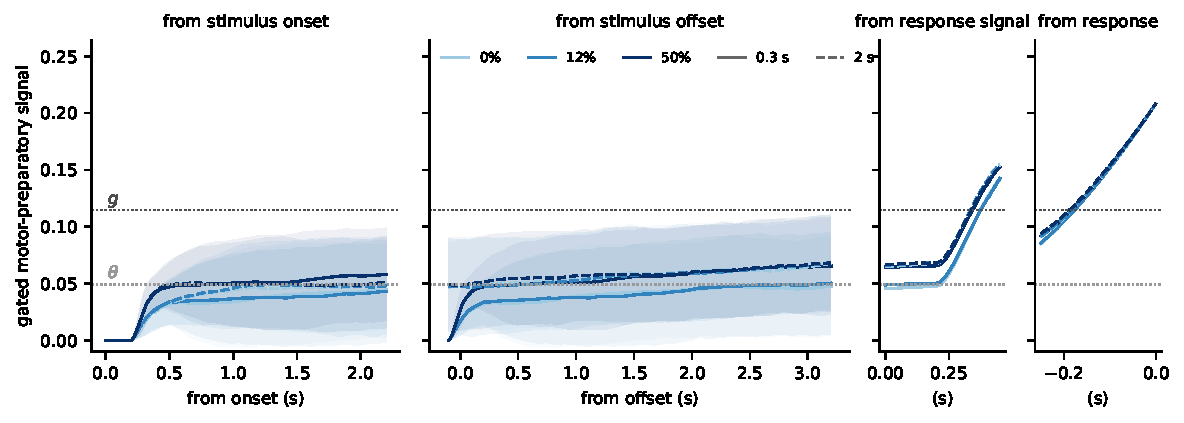
\includegraphics[width=\textwidth]{fig_traj_m2.pdf}\\[8pt]
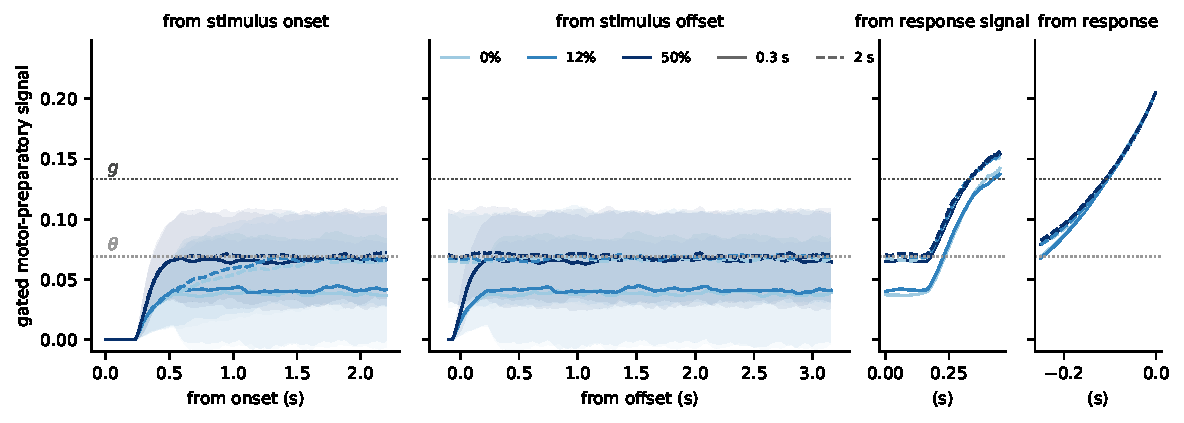
\includegraphics[width=\textwidth]{fig_traj_m1.pdf}
\caption{The manuscript's Figure~1, simulated. Mean gated motor-preparatory signal at the
calibrated parameters, time-locked to the four trial events, with a one standard
deviation band; each trial is censored at its own response. Colour is coherence, line
style is stimulus duration; the dotted lines are the internal threshold $\theta$ and the
gate $g$. Top: Model~2. Bottom: Model~1, refitted in its own right. The difference is
entirely in the second panel, where Model~2 climbs towards the gate through the delay and
Model~1 does not. The panels are means: the cartoon's clean separation between conditions
survives as an ordering, and the band shows how little of it a single trial sees.}
\label{fig:traj}
\end{figure}

\begin{figure}[p]
\centering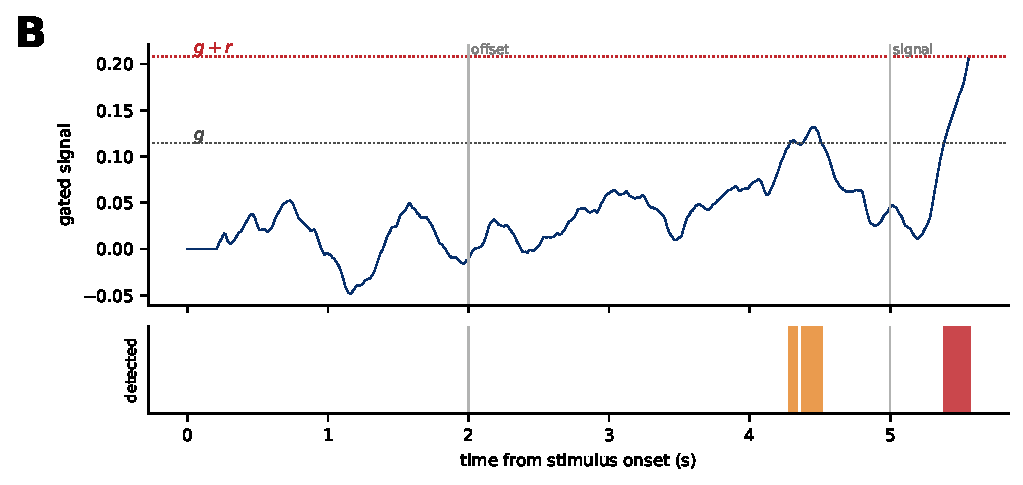
\includegraphics[width=\textwidth]{fig_single.pdf}
\caption{One simulated trial, the counterpart of the manuscript's Figure~2B--C. Above,
the gated signal with the gate $g$ and the response criterion $g+r$; below, the intervals
the detection rules return, after merging at $25$~ms and discarding intervals with too
few supra-threshold samples. Orange is a partial activation, red the activation that
reaches the criterion and becomes the response.}
\label{fig:single}
\end{figure}

\begin{figure}[p]
\centering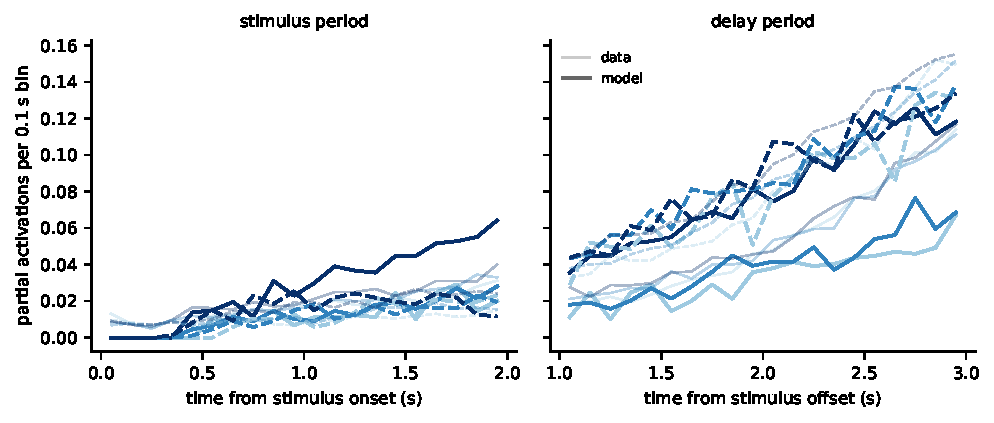
\includegraphics[width=\textwidth]{fig_rates.pdf}
\caption{Partial-activation rate, data (thin, pale) against model (thick), at the
calibrated parameters with the detection rules applied to the simulated signal. The delay
panel shows the main residual: the model spreads the three coherence levels far too
widely after a short stimulus, where the data are nearly flat. That is the saturation
argument of Section~\ref{sec:pred} made numerical.}
\label{fig:rates}
\end{figure}

\begin{figure}[p]
\centering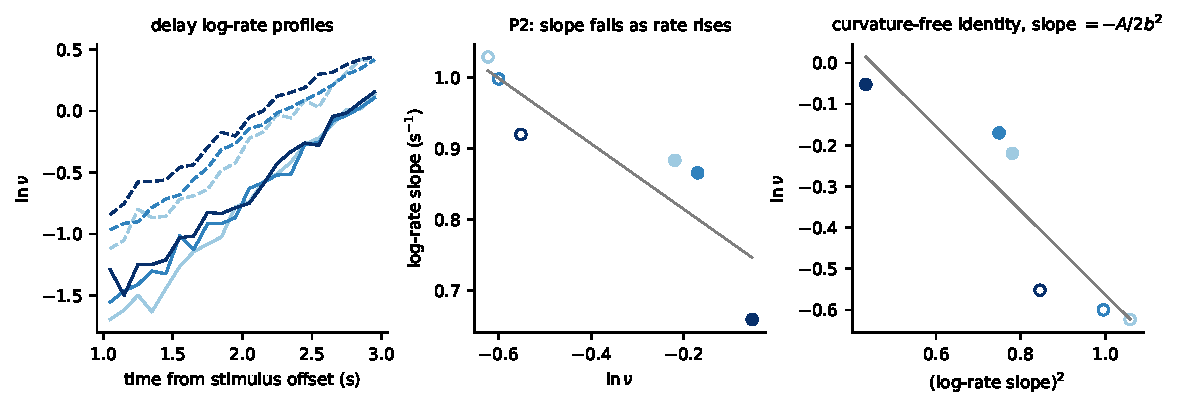
\includegraphics[width=\textwidth]{fig_shape.pdf}
\caption{The shape prediction, on data alone. Left, the six offset-locked log-rate
profiles. Right, the log-rate slope falls as the cell's rate rises, as \eqref{eq:slope}
requires, since a higher rate means a smaller distance to the gate. Open symbols are the
short duration, filled the long.}
\label{fig:shape}
\end{figure}


\appendix


\section{Tables S1 and S2, with the observations identified}
\label{app:obs}

The two tables below are Tables~S1 and~S2 of the manuscript, with one column added at the
left. A label R\emph{x} marks a result this note discusses; a blank means the result is a
null that the manuscript never mentions, and there is nothing to say about it. Values are
the true ones: where they differ from those published, the difference is flagged and
explained in the note attached to the table.

\paragraph{On the window names.} The four windows are locked to the four trial events and
do not coincide with the intervals they are named after. The onset-locked window runs from
stimulus onset to two seconds, so after a $0.3$~s stimulus it contains $0.3$~s of stimulus
and $1.7$~s of delay. That is not a detail --- it is why the duration effects in that
window separate the two models --- and it is why this note calls the windows
\emph{onset-locked}, \emph{offset-locked}, \emph{signal-locked} and
\emph{response-locked} rather than the stimulus, delay, RS and response periods. We
suggest the manuscript do the same.

\subsection*{Table S1. Accuracy, response time, premotor and motor execution time}

\begin{center}\small
\begin{tabular}{llrrrrr}
\toprule
& effect tested & df1 & df2 & $F$ & $p$ & $\eta_p^2$\\
\midrule
\multicolumn{7}{l}{\emph{Accuracy}}\\
R1 & duration & 1 & 21 & 22.68 & $<$.001 & 0.519\\
R2 & coherence & 1.31 & 27.4 & 222.22 & $<$.001 & 0.914\\
R3 & duration $\times$ coherence & 2 & 42 & 12.17 & $<$.001 & 0.367\\
\multicolumn{7}{l}{\emph{Mean response time}}\\
R4 & duration & 1 & 21 & 65.79 & $<$.001 & 0.758\\
R5 & coherence & 1.50 & 31.39 & 14.19 & $<$.001 & 0.403\\
R6 & duration $\times$ coherence & 2 & 42 & 4.61 & .016 & 0.180\\
\multicolumn{7}{l}{\emph{Mean premotor execution time}}\\
R7 & duration & 1 & 21 & 69.75 & $<$.001 & 0.769\\
R8 & coherence & 1.59 & 33.35 & 14.11 & $<$.001 & 0.402\\
R9 & duration $\times$ coherence & 2 & 42 & 3.62 & .035 & 0.147\\
\multicolumn{7}{l}{\emph{Mean motor execution time}}\\
R10 & duration & 1 & 21 & 1.03 & .320 & ---\\
& coherence & 1.51 & 31.68 & 0.54 & .537 & ---\\
& duration $\times$ coherence & 2 & 42 & 2.39 & .104 & ---\\
\bottomrule
\end{tabular}
\end{center}

\noindent\emph{Note.} Values as published; this note did not recompute them, since its
own extraction differs from the manuscript's by about a hundred trials and substituting it
would confuse a difference of analysis with a difference of data. R10 labels the three
motor-execution-time rows together: the manuscript states them as one result, that no
factor affects motor execution time, and the note treats them as one.

\subsection*{Table S2. Rate of partial activations, responding channel}

\begin{center}\small
\begin{tabular}{llrrrrr}
\toprule
& effect tested & df1 & df2 & $F$ & $p$ & $\eta_p^2$\\
\midrule
\multicolumn{7}{l}{\emph{Onset-locked window, 0 to 2 s from stimulus onset}}\\
R11 & duration & 1 & 21 & 13.38 & .001 & 0.389\\
R12 & coherence & 1.33 & 28.01 & 5.25 & .021 & 0.200\\
R13 & time & 2.70 & 56.75 & 18.05 & $<$.001 & 0.462\\
& duration $\times$ coherence & 2 & 42 & 0.312 & .734 & ---\\
R14 & duration $\times$ time & 5.09 & 106.82 & 4.645 & $<$.001 & 0.181\\
R15 & coherence $\times$ time & 38 & 798 & 1.718 & .005 & 0.076\\
& duration $\times$ coherence $\times$ time & 38 & 798 & 1.058 & .377 & ---\\
\midrule
\multicolumn{7}{l}{\emph{Offset-locked window, 1 to 3 s from stimulus offset}}\\
R16 & duration & 1 & 21 & 33.19 & $<$.001 & 0.612\\
R17 & coherence & 2 & 42 & 3.36 & .044 & 0.138\\
R18 & time & 1.21 & 25.43 & 31.42 & $<$.001 & 0.599\\
R19 & duration $\times$ coherence & 2 & 42 & 3.474 & .040 & 0.142\\
R20 & duration $\times$ time & 5.38 & 112.99 & 4.520 & $<$.001 & 0.177\\
R21 & coherence $\times$ time & 38 & 798 & 0.737 & .879 & ---\\
& duration $\times$ coherence $\times$ time & 38 & 798 & 0.959 & .542 & ---\\
\midrule
\multicolumn{7}{l}{\emph{Signal-locked window, 0 to 0.2 s from the response signal}}\\
R22 & duration & 1 & 21 & 36.56 & $<$.001 & 0.635\\
R23 & coherence & 1.56 & 32.82 & 1.159 & .315 & ---\\
R24 & time & 1 & 21 & 21.96 & $<$.001 & 0.511\\
& duration $\times$ coherence & 2 & 42 & 0.041 & .959 & ---\\
R25 & duration $\times$ time & 1 & 21 & 7.046 & .015 & 0.251\\
& coherence $\times$ time & 2 & 42 & 0.407 & .668 & ---\\
& duration $\times$ coherence $\times$ time & 2 & 42 & 0.587 & .561 & ---\\
\midrule
\multicolumn{7}{l}{\emph{Response-locked window, $-0.2$ to 0 s before the press}}\\
R26 & duration & 1 & 21 & \textbf{7.613} & \textbf{.012} & \textbf{0.266}\\
& coherence & 1.90 & 39.98 & \textbf{1.845} & \textbf{.173} & ---\\
& duration $\times$ coherence & 1.86 & 39.10 & \textbf{0.342} & \textbf{.697} & ---\\
\bottomrule
\end{tabular}
\end{center}

\noindent\emph{Note.} Values reproduce those published exactly, to the last reported
digit, except in the response-locked window, where they are printed in bold because they
differ. Two corrected data files were supplied after the note was begun. The
signal-locked window did not reproduce with the earlier file and does with the corrected
one; nothing there changes. The response-locked window changes both in value and in
shape. In the corrected file the bin from $-0.1$ to $0$~s is exactly zero for every
participant and cell --- a partial activation precedes the response burst by definition,
and the burst begins about $160$~ms before the press --- so the window carries one
informative bin, the level and trend scores are the same number up to a constant, and the
four time-related rows of the published table are not separate tests. The three effects
above are what the window supports. The main effect of duration passes from $F=0.011$,
$p=.919$ as published to $F=7.613$, $p=.012$; Section~\ref{sec:corrected} sets out the
consequences.

\subsection*{One result outside the tables}

\noindent R27, the levelling off of the rate shortly before the response signal in the
two-second, fifty-per-cent condition. It is a reading of Figure~4A rather than a row of
any table, and the manuscript discusses it at length, proposing a strategic reduction of
temporal preparation to account for it. It is labelled here because
Section~\ref{sec:pred} derives it without that mechanism.


\section{The rate of partial activations}
\label{app:nu}

Throughout, $\varphi$ and $\Phi$ are the standard normal density and distribution, and
$\rho:=t-\tau$ is elapsed maintenance time.

Define $V(t)$ on $[\tau,\trs)$ by $\dd V(t)=\lambda(\varepsilon(t)-V(t))\dd t$ with
$V(\tau)=0$, so that $y(t)=m+V(t)$. Since $\varepsilon$ admits a continuous modification
and $V$ is then a Riemann integral of a continuous function, almost surely $V\in C^{1}$,
and
\begin{equation}
V(\tau+\rho)=\int_0^\rho K(\rho-p)\,\dd B(p),
\qquad
K(v)=\frac{\lambda\sigma_\varepsilon}{\lambda-\kappa}
\bigl(e^{-\kappa v}-e^{-\lambda v}\bigr),
\label{eq:kernel}
\end{equation}
where $B$ drives $\varepsilon$, and $\varepsilon(\tau)=0$ leaves no additional
deterministic term. Note $K(0)=0$, which is what makes $V$ differentiable, and
$K'(0)=\lambda\sigma_\varepsilon$; in the degenerate case $\kappa=\lambda$,
$K(v)=\lambda\sigma_\varepsilon\,v\,e^{-\lambda v}$.

With $c:=\lambda\sigma_\varepsilon/(\lambda-\kappa)$, standard computations give
\begin{align}
\Var V(\rho)&=c^{2}\left[\frac{1-e^{-2\kappa\rho}}{2\kappa}
-\frac{2\bigl(1-e^{-(\lambda+\kappa)\rho}\bigr)}{\lambda+\kappa}
+\frac{1-e^{-2\lambda\rho}}{2\lambda}\right],\\
\Var\dot V(\rho)&=c^{2}\left[\kappa\,\frac{1-e^{-2\kappa\rho}}{2}
-\frac{2\kappa\lambda\bigl(1-e^{-(\lambda+\kappa)\rho}\bigr)}{\lambda+\kappa}
+\lambda\,\frac{1-e^{-2\lambda\rho}}{2}\right],\\
\Cov\bigl(V(\rho),\dot V(\rho)\bigr)&=\tfrac12 K(\rho)^{2}.
\end{align}
As $\rho\to\infty$,
\begin{equation}
\sigma_V^{2}=\frac{\lambda\,\mathrm{SD}_\varepsilon^{2}}{\lambda+\kappa},
\qquad
\sigma_{\dot V}^{2}=\frac{\lambda^{2}\kappa\,\mathrm{SD}_\varepsilon^{2}}{\lambda+\kappa},
\qquad
\Cov=0,
\qquad
\omega:=\frac{\sigma_{\dot V}}{\sigma_V}=\sqrt{\lambda\kappa}.
\label{eq:stat}
\end{equation}
The preparation ramp is added outside the filter, so it shifts the mean and leaves
$\sigma_V$ and $\omega$ untouched; \eqref{eq:stat} holds for both models.

On $[\tau,\trs)$, since $m=\sresp|m|$, we have
$\sresp\tilde y(t)=|m|+\sresp V(t)+\beta_t$ with
$\beta_t:=\beta(t-\toff)^{+}/\Delta$, and $\sresp V$ has the same law as $V$ because $V$
starts at zero and is driven by $W_\varepsilon$, independent of $W_x$. A partial
activation on the selected channel therefore begins exactly when $\sresp V$ crosses
\begin{equation}
d(t):=g-|m|-\beta\,\frac{(t-\toff)^{+}}{\Delta}
\end{equation}
upward. The non-selected channel activates when $\sresp V$ falls below
$-g-|m|-\beta_t$, which at the calibrated parameters is $7.1$ standard deviations away
against $1.6$ for the selected one; it is not considered further. The model therefore predicts the non-selected channel to


Denote $\nu(t)$ the upcrossing rate at time $t>\tau$ and let $Z(t):=V(t)-d(t)$, so that
upcrossings of $d$ by $V$ are upcrossings of zero by $Z$ and
$\dot Z=\dot V+\alpha$. We neglect the trajectories that reach $r$ before the end of the
delay, as these anticipations are rare, fewer than $1.5\%$ of trials, and excluded from
the empirical analysis. Since $V\in C^{1}$ and $Z$ is Gaussian and non-degenerate for
$\rho>0$, the Kac--Rice formula gives (Aza\"is and Wschebor, 2009, chapter~3)
\begin{equation}\label{eq:KR1}
\nu(t)=p_{Z(t)}(0)\,\E\left[\dot Z(t)\1_{\{\dot Z(t)>0\}}\ \middle|\ Z(t)=0\right].
\end{equation}
Since $Z(t)\sim N(-d(t),\sigma_{V}^{2})$ and $\varphi$ is even,
$p_{Z(t)}(0)=\sigma_{V}^{-1}\varphi(d(t)/\sigma_{V})$. Moreover $(Z,\dot Z)$ is jointly
Gaussian, so $\dot Z(t)\mid Z(t)=0\sim N(M_t,S_t)$ with
\begin{equation}
M_t=\alpha+\frac{\Cov(V,\dot V)}{\sigma_{V}^{2}}\,d(t),
\qquad
S_t=\sigma_{\dot V}^{2}-\frac{\Cov(V,\dot V)^{2}}{\sigma_{V}^{2}},
\end{equation}
and $\E[X\1_{\{X>0\}}]=M\Phi(M/\sqrt S)+\sqrt S\,\varphi(M/\sqrt S)$ for
$X\sim N(M,S)$. At stationarity $\Cov=0$, so $M_t=\alpha$ and $S_t=\sigma_{\dot V}^{2}$,
and dividing through by $\sigma_V$ gives, with $a:=d/\sigma_V$ and $b:=\alpha/\sigma_V$,
\begin{equation}\label{eq:KR2}
\nu(t)=\varphi\bigl(a(t)\bigr)
\left[b\,\Phi\!\left(\frac{b}{\omega}\right)
+\omega\,\varphi\!\left(\frac{b}{\omega}\right)\right],
\end{equation}
which is \eqref{eq:nu}. When $\alpha=0$ this reduces to the classical Rice formula
$\nu=(\omega/2\pi)e^{-a^{2}/2}$, and in particular $\nu\le\omega/2\pi$, attained when the
gate sits at the maintained level.



\section{Draft text for the missing Methods section}
\label{sec:methods}

The submitted manuscript has a gap on page~18, between the leakage sensitivity analysis
and the electromyographic acquisition, where the Methods for the second simulation stage
should be. What follows is draft text for that gap, together with the two additional
paragraphs the detection procedure requires. It is written to be pasted and edited, and
the numbers in it should be regenerated from the final fit.

\subsection*{Second-stage simulation: calibration to the electromyographic data}

\begin{quote}\small\itshape
The first stage established that both candidate models generate the motivating
response-time effects across broad regions of parameter space. Because behaviour alone
provided limited leverage, a second stage calibrated each model to the
electromyographic and behavioural data jointly and compared their fits.

All parameters were free, with one exception. The model is invariant under a common
rescaling of the decision variable, the motor-preparatory state, the internal threshold,
gating inhibition, the response criterion and the amplitude of maintenance fluctuations,
so the diffusion coefficient of motion-evidence accumulation was fixed at 0.100 to
define the amplitude unit. In particular the response criterion and the residual motor
latency, which the first stage inherited from immediate-report fits, were estimated here
rather than assumed; they were held constant across conditions.

Each model was fitted by minimising a normalised discrepancy over nine families of
measurements, each comprising the six coherence by duration cells: response accuracy;
the mean and interquartile range of premotor execution time; the mean and interquartile
range of motor execution time; the rate of partial muscle activations during the delay
period; the slope of the logarithm of that rate; the rate during the onset-locked window;
and the proportion of responses preceding the response signal. Each family was scaled by
the between-participant standard error of the corresponding observed value, so that
families measured in different units contributed comparably. Dispersion was quantified
by the interquartile range rather than the standard deviation because the empirical
distribution of premotor execution time has a long right tail, in 2.7\% of trials
exceeding one second, which the model does not reproduce and which would otherwise
dominate the criterion.

Stochastic differential equations were integrated with a 1-ms step, with 250 trials per
cell during the search and 900 for the reported fit, and with common random numbers
across evaluations so that the criterion was a deterministic function of the parameters.
Minimisation used the Nelder--Mead simplex in logarithmic parameter coordinates, started
from a closed-form solution obtained from the analytic relations between the observable
quantities and the parameters, and restarted with progressively larger initial simplices.

Simulated muscle activity was subjected to the same detection rules as the recorded
signal. Intervals during which the gated drive to the responding effector exceeded zero
were extracted; intervals separated by 25 ms or less were merged; merged intervals
containing fewer than three supra-threshold samples were discarded; and one partial
muscle activation was counted per surviving interval, except for the interval leading to
the response. Burst durations were not fitted, because the onset-refinement step of the
detection procedure displaces the reported boundaries by an unknown amount.

Model 1 was fitted independently rather than evaluated at the parameters obtained for
Model 2, so that the comparison would not confound the shape of the offset-locked
dynamics with their overall level.

Robustness was assessed by multiplying each free parameter in turn by 0.5 and by 2,
holding the others at their fitted values, and re-evaluating every directional
prediction; and by repeating the fit with a leak common to both accumulators at 0.25,
0.50 and 1.00 s$^{-1}$.
\end{quote}

\subsection*{Additions to the electromyographic Methods}

\begin{quote}\small\itshape
Muscle activation onsets were detected with the \texttt{myonset} package. The rectified
signal was thresholded at seven standard deviations above the baseline mean; intervals
of supra-threshold activity separated by less than 0.025 s were merged; merged intervals
containing fewer than three supra-threshold samples were discarded; and the boundaries
of each remaining interval were refined using the integrated-profile algorithm. A
partial muscle activation was defined as any detected interval other than the one
immediately preceding the button press.
\end{quote}

\noindent Two further sentences are worth adding, and are drafted here in ordinary
prose rather than as manuscript text, because whether to include them is an editorial
decision. The refinement step can only move interval boundaries earlier, so the final
event list contains activations separated by less than the merge interval; this does not
affect the counts, since the refinement does not change the number of intervals.
And $18.5\%$ of trials contain an activation ending within 25~ms of the response burst,
so response-period effects should be interpreted with the possibility of segmentation
in mind.

\section{Software}
\label{sec:software}

Two languages, split by job. Python owns the model: the simulation, the detector, the
calibration, the sweeps, the extraction of events from the archive, and the figures. R
owns the statistics: every analysis of variance, every trend decomposition, and the
Poisson analyses. They meet at two files written by \texttt{export\_for\_R.py}, holding
counts and exposures for the data and for each fitted model, so that the identical
statistical analysis runs on both sides.

The statistics exist in two interchangeable versions. \texttt{run\_stats.R} uses base R
only, with the repeated-measures machinery implemented in \texttt{rmanova.R}; it is what
produced the numbers in this note, and it exists because the analysis container cannot
reach CRAN. \texttt{run\_stats\_pkg.R} is the same analysis written with \texttt{afex},
\texttt{emmeans} and \texttt{lme4}, to be run on an ordinary machine; the values the
first version produced are listed at the end of it for comparison. The two should agree
except in the mixed-model coefficients, where a difference of a few per cent is expected
because the two-stage estimator weights participants equally and the mixed model weights
them by precision.


\end{document}
